\documentclass[oneside]{book}
\pagestyle{empty}

\usepackage{geometry}
\geometry{
	a4paper,
	top=13mm,
	left=15mm,
	right=15mm,
	bottom=15mm,
}

\usepackage[document]{ragged2e}
\usepackage{multicol}
\usepackage{amsmath}
\usepackage{wrapfig}
\usepackage{graphicx}
\usepackage{hyperref}
\usepackage{subcaption}
\usepackage[italian]{babel}
\usepackage{color}
\usepackage{listings}
\usepackage{float}
\usepackage{titlesec}

\newcommand{\NB}[1]{\medskip \textbf{N.B.}\ #1 \medskip}

\graphicspath{{immagini/}}

\definecolor{light_yellow}{RGB}{241,235,156}
\definecolor{dkgreen}{rgb}{0,0.6,0}
\definecolor{gray}{rgb}{0.5,0.5,0.5}
\definecolor{mauve}{rgb}{0.58,0,0.82}

\lstset{frame=single,
  language=Java,
  aboveskip=3mm,
  belowskip=3mm,
  showstringspaces=false,
  columns=flexible,
  basicstyle={\small\ttfamily},
  numbers=none,
  numberstyle=\tiny\color{gray},
  keywordstyle=\color{blue},
  commentstyle=\color{dkgreen},
  stringstyle=\color{mauve},
  breaklines=true,
  breakatwhitespace=true,
  tabsize=3
}

\titleformat{\chapter}[display]
{\normalfont\huge\bfseries}{}{0pt}{\Huge}
\titlespacing*{\chapter} {0pt}{-40pt}{20pt}

\begin{document}
\tableofcontents

\documentclass[oneside]{book}
\pagestyle{empty}

\usepackage{geometry}
\geometry{
	a4paper,
	top=13mm,
	left=15mm,
	right=15mm,
	bottom=15mm,
}

\usepackage[document]{ragged2e}
\usepackage{multicol}
\usepackage{amsmath}
\usepackage{wrapfig}
\usepackage{graphicx}
\usepackage{hyperref}
\usepackage{subcaption}
\usepackage[italian]{babel}
\usepackage{color}
\usepackage{listings}
\usepackage{float}
\usepackage{titlesec}

\definecolor{light_yellow}{RGB}{241,235,156}
\definecolor{dkgreen}{rgb}{0,0.6,0}
\definecolor{gray}{rgb}{0.5,0.5,0.5}
\definecolor{mauve}{rgb}{0.58,0,0.82}

\lstset{frame=single,
  language=Java,
  aboveskip=3mm,
  belowskip=3mm,
  showstringspaces=false,
  columns=flexible,
  basicstyle={\small\ttfamily},
  numbers=none,
  numberstyle=\tiny\color{gray},
  keywordstyle=\color{blue},
  commentstyle=\color{dkgreen},
  stringstyle=\color{mauve},
  breaklines=true,
  breakatwhitespace=true,
  tabsize=3
}

\titleformat{\chapter}[display]
{\normalfont\huge\bfseries}{}{0pt}{\Huge}
\titlespacing*{\chapter} {0pt}{-40pt}{20pt}

\begin{document}
\tableofcontents

\chapter{lambda expression}
\chapter{Stream}

Sono una “vista” dei dati per specificare computazioni a un più alto livello concettuale rispetto alle collezioni e gli iteratori.

Supponiamo di voler calcolare la media dei salari di una collezione di oggetti Employee.
\begin{multicols}{2}
Se decidessimo di usare gli iteratori
\begin{itemize}
    \item dovremmo dichiarare una variabile per accumulare i risultati intermedi;
    \item iterare sulla sorgente dati, dove, ad ogni iterazione, aggiorniamo i risultati intermedi;
    \item alla fine, calcolare la media.
\end{itemize}
\columnbreak
Se usassimo gli stream, basterebbe
\begin{itemize}
    \item specificare la sorgente dati;
    \item la proprietà di interesse;
    \item cosa vogliamo fare con quella proprietà.
\end{itemize}
La libreria stream farà tutto il resto ottimizzando il calcolo.
\end{multicols}

Rispettano il principio "what, not how", ovvero si specifica cosa si vuole fare e non il come deve essere fatto. 

Stream e collezioni, superficialmente, sembrano simili, entrambi permettono di trasformare e recuperare dati ma 
\begin{itemize}
    \item uno stream non \underline{memorizza} i dati, sono memorizzati nella collezione originale o generati su richiesta;
    \item uno stream non \underline{modifica} i dati originali, ma genera un nuovo stream dove alcuni elementi dello stream precendete non sono presenti nello 
    stream corrente;
    \item le operazioni sono \underline{lazy}, ovvero non vengono eseguite finché non serve il risultato.
\end{itemize}

Gli stream si basano sul \underline{method chaining}, ovvero chiamano un metodo sul risultato di un altro metodo, senza memorizzare i risultati intermedi.

Il workflow tipico di uno stream consiste nel creare una "pipeline" di operazioni divise in tre fasi:
\begin{itemize}
    \item creazione dello stream;
    \item specifica delle operazioni intermedie;
    \item applicazione di un’operazione finale di riduzione, per produrre un risultato, oppure un'operazione di raccolta.
\end{itemize}

\section{Creazione di uno stream}

Gli stream si creano da collezioni e array o usando generatori o iteratori.
\smallskip

Per le collezioni abbiamo i metodi stream() e parallelStream(), per gli array o un numero arbitrario di argomenti (vararg) abbiamo il metodo statico Stream.of() 
e poi abbiamo i metodi Stream.generate(Supplier $<$T$>$) e\newline Stream.iterate(T seed, UnaryOperator$<$T$>$ f).

Gli ultimi due metodi possono genera stream infiniti.

\subsection{Stream infiniti}
Stream.generate(Supplier $<$T$>$) prende una lambda senza argomenti e viene chiamato solo quando viene richiesto allo stream il prossimo elemento
\begin{lstlisting}
Stream<String> echos = Stream.generate(() -> "Echo");
Stream<Double> randoms = Stream.generate(Math::random); 
\end{lstlisting}

Stream.iterate(T seed, UnaryOperator$<$T$>$ f) prende una lambda dove seed è il "seme" iniziale mentre f è una funzione che sarà applicata al valore precendete
\begin{lstlisting}
Stream<BigInteger> integers = Stream.iterate(BigInteger.ZERO, n -> n.add(BigInteger.ONE))   
\end{lstlisting}

\section{Operazioni intermedie}

Le operazioni intermedie di uno stream sono metodi che trasformano lo stream in un altro stream, per esempio filter() che si occupa di filtrare uno stream, map()
che si occupa di trasformare gli elementi di uno stream, limit() che limita ad un certo numero di elementi dello stream (occhio a dove lo mettiamo), skip() che salta 
determinati elementi dello stream, distinct() che scarta i duplicati, etc\dots
\smallskip

Con gli stream si scrive meno codice, lo si rende più leggibile ma allo stesso tempo è molto facile commettere errori, i due prossimi stream forniscono un risultato 
differente

\begin{lstlisting}
#SI LIMITA ALLE PRIME 5 STRINGHE CHE RISPETTANO IL FILTRO
long count = words.stream()
                    .filter(w -> w.length() > 12)
                    .limit(5)
                    .count();
#SI LIMITA ALLE PRIME 5 STRINGHE                    
long count = words.stream()
                    .limit(5)
                    .filter(w -> w.length() > 12)
                    .count();
\end{lstlisting}

\section{Operazione di riduzione di uno stream}

Una volta applicate tutte le operazioni di trasformazione, alla fine si deve applicare un’operazione di riduzione.

Alcuni metodi di riduzione sono min() e max() che restituiscono, rispettivamente, il minimo ed il massimo di uno stream in base ad un criterio oppure il metodo 
reduce(\dots) che prende una funziona binaria e continua ad applicarla partendo dai primi due elementi.
\begin{lstlisting}
List<Integer> values = ...;
Optional<Integer> sum = values.stream().reduce((x, y) -> x + y);
\end{lstlisting}

Le operazioni di raccolta/riduzione forzeranno l’esecuzione di tutte le operazioni precedenti e dopo ciò lo stream non potrà più essere usato.

Alcuni di queste operazioni, come reduce(\dots), restituiscono un oggetto di classe Optional, un’alternativa più sicura della gestione dei valori null come ad esempio 
findFirst(), ifPresent(), etc\dots

\subsection{Optional}
Un oggetto Optional$<$T$>$ è un wrapper di un oggetto T oppure nessun oggetto.

L'idea di base sull’utilizzo di un oggetto Optional è quella di usare i suoi metodi che permettono di produrre un’alternativa se il valore non è presente o consumarlo.

Questo oggetto deve essere usato in modo appropriato, altrimenti si hanno gli stessi problemi che si hanno con null, ad esempio
\begin{lstlisting}
Optional<T> optionalValue = ...;
optionalValue.get().someMethod();

T value = ...;
value.someMethod();
\end{lstlisting}

Questi due blocchi sono uguali, se optionalValue non contenesse alcun valore, allora avremo una NPE, stessa cosa per quest'altro esempio
\begin{lstlisting}
if (optionalValue.isPresent())
    optionalValue.get().someMethod();

if (value != null)
    value.someMethod();
\end{lstlisting}




\section{Operazione di raccolta di uno stream}

Un'alternativa alla riduzione di uno stream è la raccolta, ci sono molti metodi tra cui il metodo collect() che prende in input oggetti che implementano l'interfaccia
Collector, tra cui Collectors che fornisce metodi per creare istanze delle collezioni più comuni come ad esempio toList() o toSet(), iterator() che ritorna un iteratore
o anche toArray().

Spesso si vuole una mappa che associa ad una chiave, una collezione di oggetti e qui entrano in gioco i metodi di raggruppamento o partizionamento.

Si usa il primo specificando la lambda che calcola la chiave, detta \textit{classifier function} mentre si usa il secondo quando quest'ultima è booleana
\begin{lstlisting}
#per ogni stringa del nome abbiamo la lista delle relative persone
Map<String, List<Person>> sameName = people.collect(Collectors.groupingBy(Person::getName));

#abbiamo due liste, una che contiene il nome e una che non lo contiene
Map<Boolean, List<Person>> emptyNames = people.collect(Collectors.partitioningBy(p -> p.getName().isEmpty()));
\end{lstlisting}

Di default groupingBy raggruppa in una List ma ci sono altre versioni che permettono di specificare un downstream collector
\begin{lstlisting}
#visto prima
Map<String, List<Person>> sameName = people.collect(Collectors.groupingBy(Person::getName));

#nuovo tipo
Map<String, Long> sameName = people.collect(Collectors.groupingBy(Person::getName, Collectors.counting()));
\end{lstlisting}

\end{document}

\chapter{INFORMATION HIDING}

Utilizzo di meccanismi per evitare che tutti possano accedere a certe parti di codice.\\
Noi abbiamo visto i livelli di accessibilità in Java

\begin{figure}[H]
  \centering
  \includegraphics[width=0.5\linewidth]{../../immagini/information_hiding/accessibilità}
\end{figure}

Per convenzione

\begin{itemize}
  \item le variabili d'instanza dovrebbero essere private (evita anche protected);
  \item i campi static, per rappresentare costanti accessibili a tutti, dovrebbero essere public final;
  \item i metodi che utilizzano dettagli interni dovrebbero essere private;
  \item i metodi che potrebbero servire alle sottoclassi, dovrebbero essere protected;
  \item i metodi che saranno usati dalle altre classi, dovranno essere public.
\end{itemize}

Creare un oggetto che ha parametri d'instanza, privati, che però vi si possonono accedere, con un get, o settare, tramite un setter, è la cosa sbagliata.\\
Supponiamo di avere una classe Person tale che

\begin{lstlisting}
  public class Person {
    private String name;
    
    public Person(String name) {
      this.name = name;
    }
    
    @Override
    public String toString() {
      return "Person [name=" + name + "]";
    }
}
\end{lstlisting}

Se instaziassi la classe e cercassi di accedere al campo name, il compilatore mi segnalerebbe errore.\\
L'information hiding è pensato per essere usato a tempo di compilazione e non a run time.\\
Java permette di accedere alle variabili, anche private, di una classe.\\
infatti

\begin{lstlisting}
  @Test public void testReadPrivateMember() throws ... {
    Person person = new Person("John");
    // riferimento al campo (anche se privato)
    Field nameField = person.getClass().getDeclaredField("name");
    // aggira il controllo di accesso
    nameField.setAccessible(true);
    // legge il valore del campo
    Object nameValue = nameField.get(person);
    assertEquals("John", nameValue);
  }
\end{lstlisting}

\textbf{N.B.} Il metodo setAccessible(boolean bol) permette, effettivamente di accedere ai campi private, altrimenti non sarebbe possibile farlo.\\
Se io dichiarassi name public, legittimerei il suo uso da parte dei cliente, imponendomi il vincoli non poter mai più modificare quella variabile, altrimenti i client verranno rotti (non compileranno più).\\
Ogni client che userà quel membro sarà strettamente accoppiato (tightly coupled) a quel membro (noi questo non lo vogliamo).\\
Stessa cosa per protected, solo che qui saranno le sottoclassi ad essere tightly coupled.\\
Dichiarando un membro private, lo nascondo al "mondo", non legittimiamo il suo uso da parte dei client.\\
Il compilatore controllerà il corretto uso nei vari client e

\begin{itemize}
  \item se compileranno con errori di accesso, significa che i client non sono legittimati all’uso;
  \item se accederanno al membro via reflection (run time) e qualcosa non dovesse funziona, sarà colpa loro. 
\end{itemize} 

Più dettagli interni nascondiamo, più avremo disaccoppiamento e più sarà facile testare singole componenti in isolamento.\\
Se diachiarassimo qualcosa come public/protected, come le API, e volessimo effettuare dei cambiamento, dovremmo notificare i client quando rilasceremo il nuovo aggiornamento, specificando se si tratta di qualcosa che rompe API, implementa qualcosa di nuovo oppure la risoluzione di bug.\\
Un modo per indicare questi cambiamenti è l'utilizzo della semantic versioning, un numero composta da tre parti, $X.Y.Z$, dove se

\begin{itemize}
  \item dovesse cambiare X, significherebbe aver introdotto qualcosa che rome l'API;
  \item dovesse cambiare Y, significherebbe aver introdotto qualcosa di nuovo;
  \item dovesse cambiare Z, significherebbe aver risolto dei bug (sperando di non aver introdotto nuovi bug).
\end{itemize}

\section{Design Pattern VS Design Principle}

Un design pattern sbalisce la linea guida su cosa è giusto e su cosa è sbagliato quando si fa il design di un’applicazione, dice cosa fare (e non fare) e non come farlo.

Un design principle è una soluzione generica e riusabile per un problema comune, dicono come risolvere un problema in un certo contesto software, fornendo chiare linee guida.

\chapter{ACRONIMO SOLID}

I principi SOLID prescrivono come organizzare funzioni e dati in classi e come tali classi dovrebbero essere interconnesse.

Lo scopo di questi principi è la creazione di strutture software che tollerano il cambiamento, sono facili da comprendere/testare e sono riusabili in diversi sistemi software.

\section{Single Responsability Principle (SRP)}

Prevede che una classe deve avere una sola responsabilità, ovvero deve avere una e una sola ragione per essere modificata.

Si dice che la classe deve essere 

\begin{itemize}
  \item \textit{coesiva}, ovvero quanto le cose di un certo gruppo hanno ragione di stare insieme;
  \item \textit{loosely coupling}, ovvero deve dipendere il meno possibile dai metodi di altre classi.
\end{itemize}

Se una classe è responsabile di più cose, la si dovrà cambiare più spesso e cambiare frequentemente una classe porta ad avere ripercussioni su tutte quelle classi che dipendono da lei.

Ciò comporterà, ad ogni modifica, nuova ricompliazione e nuovo test dei metodi.

Prima di aggiungere qualcosa di nuovo a una classe ci si dovrebbe interrogare su quale sia la responsabilità di questa classe, se la risposta comprende funzionalità scorrelate congiunte
con un “e” o un “oppure” allora, probabilmente, si sta violando l’SRP.

\section{Open-Closed Principle (OCP)}

Il principio aperto/chiuso stabilisce che le classi debbano essere aperte alle estensioni e chiuse alle modifiche.

Per modifica si intende il cambiamento del codice di una classe esistente ed estensione significa aggiungere nuove funzionalità.

Tutto ciò sta a significare che dovremmo essere in grado di aggiungere nuove funzionalità senza toccare il codice attuale della classe, questo perché ogni volta che modifichiamo il codice,
rischiamo di dare vita a potenziali bug.

Se nell'SRP si cerca di decomporre la responsabilità, qui si cerca di capire quali parti devono essere concrete (da implementare) e quali devono essere astratte (saranno implementate dai 
consumatori del software).

Negli OOP abbiamo a disposizione il meccanismo dell'ereditarità per creare una classe derivata da una già esistente, il meccanismo dell'override per ridefinire un metodo della classe 
padre e la funzionalità del binding dinamico che permette, dato un oggetto, di chiamare il metodo giusto a runtime.

Questo, però, non è detto che basti a rispettare OCP, specialmente se si estende una classe concreta o se la classe derivata si basa, fortemente, su dettagli implementatitivi della superclasse.
Per esempio, voglio estendere una classe, MySet, per contare gli elementi inseriti

\begin{multicols}{2}
  \begin{lstlisting}
    public class MySet<E> {
      public void add(E o) {
      // add the element to the internal set
      }

      public void addAll(Collection<E> c) {
        for (E e : c) {
          add(e);
        }
      }
    }
  \end{lstlisting}
  \columnbreak
  \begin{lstlisting}
    public class MyCountingSet<E> extends MySet<E> {
      private int count = 0;
      
      @Override
      public void add(E o) {
        super.add(o);
        count++;
      }
    } 
  \end{lstlisting}
\end{multicols}

\newpage
Se io modificassi MySet, ad esempio modifico addAll(), non chiamando più dentro add(), allora la mia classe derivata non sarebbe più corretta, in quanto non avremo più un aumento del contatore.

Quindi, per risolvere questo problema, devo modificare la mia classe, facendo override anche del secondo metodo

\begin{multicols}{2}
  \begin{lstlisting}
    public class MySet<E> {
      public void add(E o) {
      // add the element to the internal set
      }

      public void addAll(Collection<E> c) {
        // add directly all elements
        // WITHOUT relying on add
      }
    }
  \end{lstlisting}
  \columnbreak
  \begin{lstlisting}
    public class MyCountingSet<E> extends MySet<E> {
      private int count = 0;
      
      @Override
      public void add(E o) {
        super.add(o);
        count++;
      }

      @Override
      public void addAll(Collection<E> c) {
        super.addAll(c);
        count += c.size();
      }
    } 
  \end{lstlisting}
\end{multicols}

Inoltre, se ad un certo punto tornassi alla versione originale di MySet, avrei lo stesso problema, ovvero MyCountingSet non funzionerebbe più in quanto il contatore verrebbe incrementato due 
volte ogni volta.

Quindi possiamo vedere che le modifiche fatte a MySet possono anche essere giuste o minimali ma sono devastanti per la mia sottoclasse.

Questo porta al concetto della \textbf{fragile base class problem}, ovvero una classe è considerata fragile se piccole modifiche corrette e sicure alla classe base, possono portare le classi 
derivate a non funzionare più correttamente.

Quindi sarebbe meglio proibire l'estensione della classe (con un final), proibire la ridefinizione di alcuni metodi (anche qui final) e documentare come una classe base dovrebbe essere usata/estesa.

Allora, dal concetto di classi concrete ed ereditarietà, arriviamo al concetto di classi astratte o interfacce ed, eventualmente, al principio di composizione e delega.

\begin{wrapfigure}{r}{3cm}
  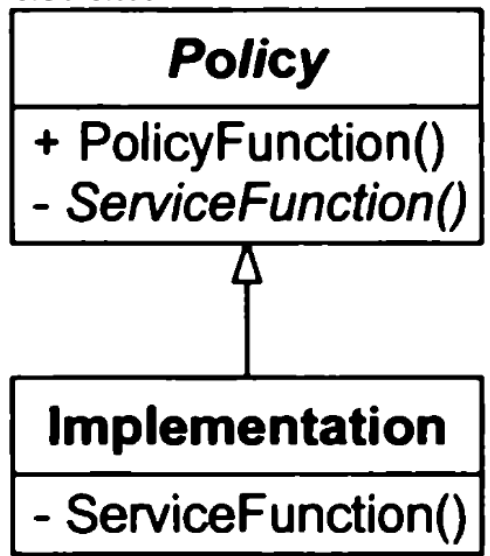
\includegraphics[width=0.5\linewidth]{../../immagini/principio_SOLID/esempioOCP}  
\end{wrapfigure}

Prediamo come esempio la classe astratta Policy che ha un metodo, public e probabilmente final, PolicyFunction che, a sua volta, implementa una certa politica in termini di un metodo, protetto e 
astratto, ServiceFunction.

Policy, quindi, ha una parte concreta (PolicyFunction) ed una astratta (ServiceFunction), si dice che è aperta all'estensione, tramite la parte astratta e chiuse alle modifiche dovute al fatto 
che PolicyFunction è final.

Supponiamo di avere una classe Client che si occupa di fare logging e di voler aggiungere un nuovo tipo di log, basterà, quindi, aggiungere un nuovo tipo di logging ad enum ed un nuovo ramo allo if-else.

Come si vede, la classe è si configurabile rispetto al log ma non è aperta ad estensioni del log in quanto la sua gestione dipende da un if-else/switch e quanfo si usa un if-else/switch, si sta violando 
OCP, inoltre c'è il dubbio su cosa faccia l'ultimo else (in questo caso non fa nulla).

\begin{lstlisting}[linewidth=10cm]
public class Client {
  public enum LogConf { CONSOLE, FILE }
  private LogConf logConf;
  
  public Client(LogConf logConf) { this.logConf = logConf; }
  
  public void aMethod() {
    // do something before or after the log method...
    log("a message");
  }

  private void log(String message) {
    if (logConf == LogConf.CONSOLE) {
    // log to System.out
    } else if (logConf == LogConf.FILE) {
    // log to a File
    } else {
    // what to do?!?
    }
  }
}
\end{lstlisting}

\newpage
Quindi, per risolvere ciò
\begin{itemize}
  \item decidiamo di astrarre la funzionalità di logging attraverso l'interafccia Log che avrà diverse implementazioni come ConsoleLog o FileLog;
  \item la classe Client dichiara una variabile privata di tipo Log;
  \item l’istanza Log viene passata al costruttore;
  \item Client delega completamente il logging all’istanza di Log.
\end{itemize}

La nuova classe è estendibile a nuovi sistemi di logging, infatti basta creare una nuova implementazione di Log, il Client non è stato minimamente toccato, non c'è stato bisogno di ricompilare.

\begin{multicols}{2}
  \begin{lstlisting}
    public class Client {
      private Log logger;
        
      public Client(Log log) {
        this.logger = log;
      }
        
      public void aMethod() {
        // do something...
        log("a message");
        // do something...
      }
    
      private void log(String message) {
        logger.log(message);
      }
    }
  \end{lstlisting}
  \columnbreak
  \begin{lstlisting}
    public interface Log {
      public void log(String message)
    }

    public class ConsoleLog implements Log {...}

    public class FileLog implements Log {...}
  \end{lstlisting}  
\end{multicols}
Ovviamente le due classi concrete fanno override del metodo log.\\
Esempio pratico sono i software basati sui plug-in, ovveri software che non è possibile modificare ma estendibili tramite plug-in.\\

\section{Liskow Substitution Principle (LSP)}
 
Questo principio si basa sul concetto di sottotipo.

In java, un oggetto di tipo T sottotitpo di S, detto supertipo, può essere sempre
\begin{itemize}
  \item assegnato a una variabile dichiarata di tipo S;
  \item passato come argomento di un metodo che si aspetta un parametro di tipo S;
  \item restituito in un metodo il cui tipo di ritorno è S.
\end{itemize}

Per un sottotitpo valgono la proprietà riflessiva, ovvero data una classe A, A è sottotipo di se stessa (si indica con $A<:A$) e la proprietà transitiva, ovvero siano 
A, B e C tre classi, se $A<:B$ e $B<:C\Rightarrow A<:C$.

Il prinicipio di Liskow è qualcosa di più forte della definizione di sottotipo, ovvero, vuole che il comportamento del programma, quando sostituisco S con T, non 
cambia, non si rompe, continua a funzionare correttamente (non significa che non cambia nulla, altrimenti non avrebbe senso).

Per esempio, ho una classe Rectangle con due campi, height e weight, metodi setter ed un metodo area.
\begin{multicols}{2}
  \begin{lstlisting}
  public class Rectangle {
    private int height, width;
    
    public void setHeight(int height) {...}

    public void setWidth(int width) {...}

    public int area() { return height * width;}
  }
  \end{lstlisting}
  \columnbreak
  \begin{lstlisting}
    @Test
    public void testRectangle() {
      Rectangle r = new Rectangle();
      r.setHeight(5);
      r.setWidth(3);
      assertEquals(15, r.area());
    }
  \end{lstlisting}
\end{multicols}

Ora voglio creare la classe Square da rettangolo, tanto basta porre entrambi i lati uguali.\\
\begin{multicols}{2}
  \begin{lstlisting}
    public class Square extends Rectangle {
      
    @Override
      public void setHeight(int height) {
        super.setHeight(height);
        super.setWidth(height);
      }

      @Override
      public void setWidth(int width) {
        super.setWidth(width);
        super.setHeight(width);
      }
    }
  \end{lstlisting}
  \columnbreak
  \begin{lstlisting}
    @Test
    public void testSquare() {
      Square s = new Square();
      s.setHeight(5);
      assertEquals(25, s.area());
      s.setWidth(3);
      assertEquals(9, s.area());
    }
  \end{lstlisting}
\end{multicols}  

Presi singolarmente, i test passano, ora, però, bisogna vedere che, se applicando il principio di sostituzione, tutto rimane invariato.\\
\begin{lstlisting}[linewidth=8cm]
  @Test
  public void testSquareAsRectangle() {
    Rectangle r = new Square();
    r.setHeight(5);
    r.setWidth(3);
    assertEquals(15, r.area());
  }
\end{lstlisting}

Questo test fallisce perchè, quando chiamo in sequenza i due metodi setter, questi saranno chiamati da quadrato e non da rettangolo (binding dinamico).

Quindi Square non è sostituibile a Rectangle anche perchè alla classe Square, alla fine dei conti serve un solo campo.

Per risolvere il problema possiamo pensare di eliminare i due metodi setter ed introdurre un'interafccia, Shape, con all'interno la definizione del metodo area.

Così facendo, entrambe le classi concrete, implementeranno Shape e ridefineranno, a modo loro, il metodo area attraverso override.

\begin{center}
  \begin{tabular}{c}
    \begin{lstlisting}[linewidth=5cm]
      public interface Shape {
        public int area();
      }
  \end{lstlisting}
  \end{tabular}
\end{center}

\begin{multicols}{2}
  \begin{lstlisting}
    public class Rectangle implements Shape {
      private int height, width;
      
      public Rectangle(int height, int width) {
        this.height = height;
        this.width = width;
      }

      @Override
      public int area() { return height * width;}
    }
  \end{lstlisting}
  \columnbreak
  \begin{lstlisting}
    public class Square implements Shape {
      private int side;
      
      public Square(int side) {
        this.side = side;
      }
      
      @Override
      public int area() { return side * side;}
    }
  \end{lstlisting}
\end{multicols}

I test che useranno Shap, passandogli prima Rectangle e poi Square, funzioneranno
\begin{lstlisting}[linewidth=6cm]
  @Test
  public void testShape() {
    Shape s = new Rectangle(5,3);
    assertEquals(15, s.area());
    s = new Square(5);
    assertEquals(25, s.area());
  }  
\end{lstlisting}

Detto in parole povere, bisogna cercare di lavorare, il più possibile, con classi astratte o interfacce, lavorare verso l'astrazione e non verso l'implementazione.

\newpage
\section{Iterafce Segregation Principle (ISP)}

È simile all’SRP ma incentrato su interfacce e client.

Supponiamo di avere a disposizione un'interfaccia contente metodi che svolgono differenti compiti.

Un client che implementerà questa interfaccia, sarà costretto ad implementare tutti i suoi metodi, anche quelli che non gli servono.

Se un client richiedesse una modifica all’interfaccia, anche gli altri client ne sarebbero influenzati, anche se la modifica dovesse riguardare un metodo che a loro
non serve.

Quindi sarebbe conveniente dividere l'interfaccia originale in interfacce più piccole, così facendo l'interfaccia originale conterrà solo i metodi comuni ai client, 
mentre le interfacce più piccole si occuperanno dei metodi specifici.

Prendiamo ad esempio il sistema di pagamento di un parcheggio

\begin{lstlisting}[linewidth=15cm]
  public interface Parcheggio {

    void parcheggiaAuto();	// Diminuisce parcheggi vuoti di 1
    void esceAuto(); // Aumenta parcheggi vuoti di 1
    void getCapienza();	// Restituisce capienza auto
    double calcolaQuota(Auto auto); // Restituisce il prezzo in base al numero di ore
    void faiPagamento(Auto auto);
  }

  class Auto {
    ...
  }
\end{lstlisting}

Immaginiamo di voler implementare un parcheggio gratuito (che estenderà Parcheggio) e notiamo che abbiamo obbligato questa classe ad implementare i metodi di pagamento
del parcheggio anche se non ne avrebbe bisogno (è gratis) e magari, nel metodo pagamento, lanciamo un'eccezione gestita con un semplice "il parchegio è gratis".

Quindi si nota che l'interfaccia Parcheggio si occupa di due logiche distinte, quella del parcheggio e quella del pagamento del parcheggio stesso.

Una possibile soluzione, quindi, sarebbe quella di scindere l'interfaccia parcheggio in altre due interfacce, quella a pagamento e quella gratis, la prima oltre 
ad ereditare i metodi riferiti al parcheggio, aggiungerà i metodi riguardanti i pagamenti, mentre la seconda, implementrà l'interfaccia padre.

Con questo nuovo modello, possiamo anche andare oltre e dividere l'interfaccia pagamento per supportare diverse modalità di pagamento.

\begin{figure}[H]
  \centering
  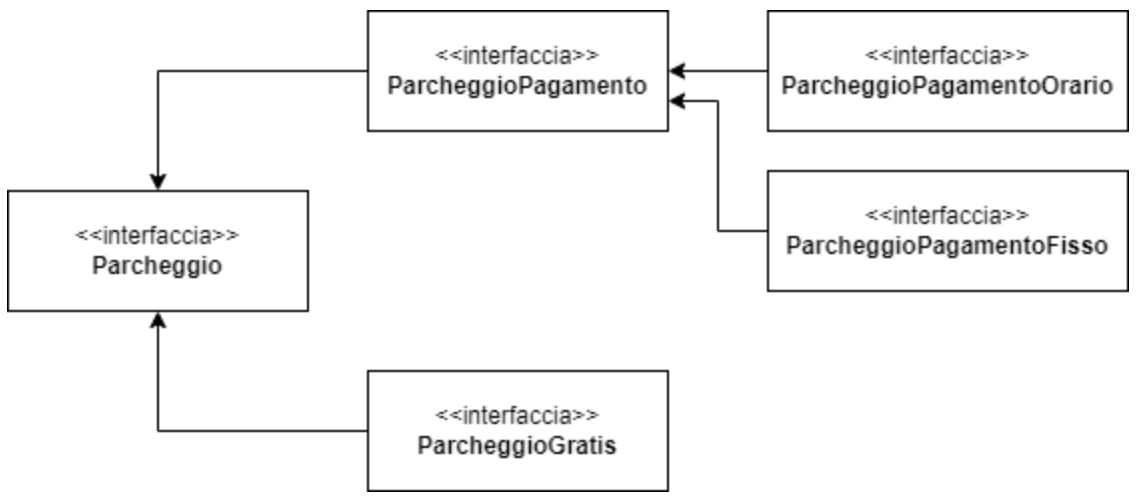
\includegraphics[width=0.5\linewidth]{../../immagini/principio_SOLID/refactoring_interfaccia.png}
\end{figure}

\section{Dependency Inversion Principle (DIP)}

Questo principio ci dice che i sistemi più flessibili sono quelli dove le dipendenze del codice sorgente si riferiscono solo alle astrazioni.

Per dipendenza nel codice sorgente si intende che, dato un file Client.java, se in dato file nomino un tipo A, allora diremo che il codice sorgente di Client dipende 
da A, anche se dovessimo usare un sottotipo di A, B, diremo che Client dipende, staticamente, da A.

Da qui utilizzeremo il concetto di modulo/componente inteso come raggruppamento di classi.

Tradizionalemente, i moduli di alto livello dipendono dai moduli di basso livello, per dipendere si intende chiamare direttamente codice di basso livello o istanziare
direttamente classi concrete.

Per codice di alto livello, detto anche core, intendiamo la parte di un'applicazione computazionale, algoritmica o che elabora, ovvero è la parte che contraddistingue 
un'applicazione.

Mentre per codice di basso livello intendiamo interfaccia utente o database.

Quindi se il codice di alto livello dipende dal codice di basso livello, significa che modifiche a quest'ulitmo, avranno un impatto sul codice di alto livello.

\newpage
Si prende come esempio un'architettura OO dove la parte più alta indica codice di alto livello.
\begin{wrapfigure}{r}{8cm}
  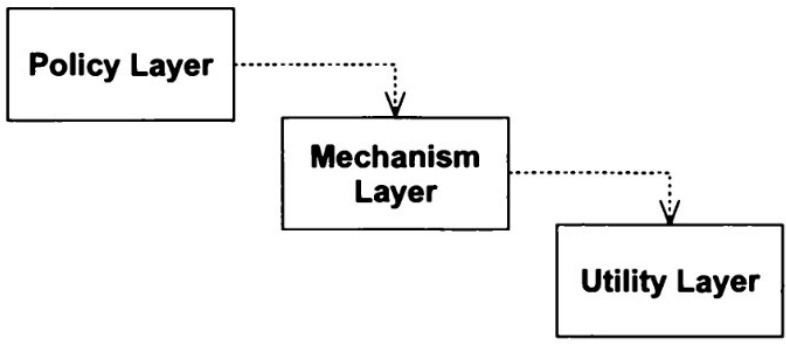
\includegraphics[width=0.5\linewidth]{../../immagini/principio_SOLID/architetturaOOnoDIP}  
\end{wrapfigure}

Il layer di alto livello usa solo il layer sottostante ma usare significa che dipende dal layer sottostante.

Inolte se il layer sottostante dipende dal layer di basso livello, allora il layer di alto livello, transitivamente, dipende dal layer di basso livello.

Per risolvere questo problema
\begin{itemize}
  \item ogni layer di alto livello dovrebbe dichiarare una propria interfaccia per i servizi di cui ha bisogno e farla implementare al layer sottostante;
  \item il layer sottostante implementerà l'interfaccia dichiarata dal layer superiore.
\end{itemize}

Così facendo, le dipendenze vengono invertite, ovvero sono i layer di basso livello a dipendere dai layer di alto livello.
\begin{figure}[H]
  \centering
  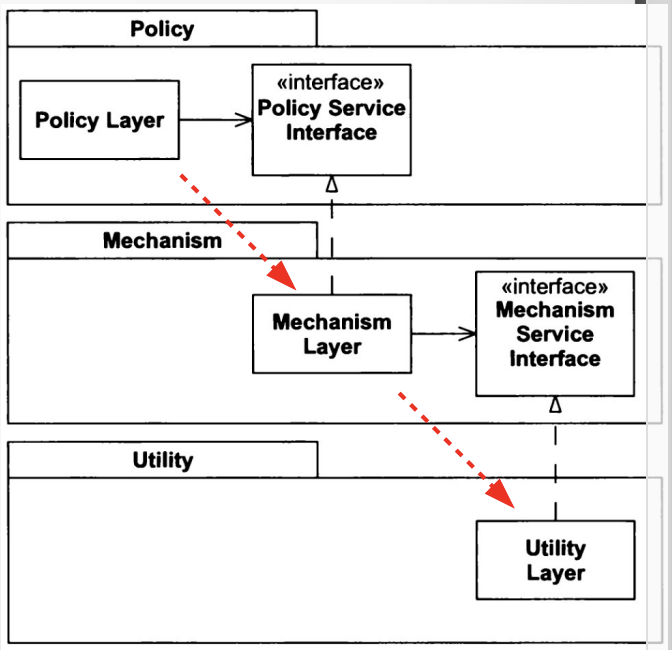
\includegraphics[width=0.35\linewidth]{../../immagini/principio_SOLID/architetturaOODIP}  
\end{figure}

staticamente Policy chiama un metodo dell'interfaccia, a runtime verrà invocato l'implementazione di tale metodo dal layer inferiore, così facendo, posso cambiare un
layer sottostante senza modificare un layer soprastante e posso testare un layer soprastante senza avere un layer sottostante ed inoltre è buona cosa non menzionare 
mai il nome di qualcosa che è concreto (non astratto) e volatile (che cambia spesso) e non avervi riferimento.

Quindi, i design pattern guidano lo sviluppo del codice e il refactoring aiutando a sviluppare software pulito e facile da estendere, riusare, mantenere e testare.

\chapter{COVARIANZA E CONTROVARIANZA}

Dalla matematica, una funzione \textit{f}, tale che f$:D\rightarrow C$, può essere sosituita da una funzione \textit{g}, tale che g$:D^\prime\rightarrow C^\prime$, sse $C^\prime<:C$ 
(\textbf{covariante} sul tipo di \textbf{ritorno}) e $D<:D^\prime$ (\textbf{controvariante} su tipo del \textbf{parametro}), ovvero una funzione g, che deve 
sostituire f, può essere più specifica sul tipo di ritorno e più generale sul parametro in input.

Supponiamo di avere due classi, Employee e Manager, tale che Manager$<:$Employee.

Employee ha un metodo setSalary() e Manager ha il metodo setBonus(int).

Prendiamo altre due classi, EmployyeDB e ManagerDB, tale che ManagerDB$<:$EmployyeDB.

La prima ha al suo interno un metodo find(int) che restiusce un Employee, mentre il secondo ridefinisce il metodo facendo tornare un Manager.
\begin{multicols}{2}
    \begin{lstlisting}
    public class EmployeeDatabase {
        public Employee findEmployee(int id) {
            ...
        }
    }    
    \end{lstlisting}       
\columnbreak
    \begin{lstlisting}
    public class ManagerDatabase extends EmployeeDatabase {
        @Override
        public Manager findEmployee(int id) {
            ...
        }
    }
    \end{lstlisting}
\end{multicols}

Se eseguissi questo codice, tutto funzionerebbe.

\begin{lstlisting}
    EmployeeDB d = new ManagerDB();
    Employee e = d.find(1);
\end{lstlisting}

Per il binding dinamico, d staticamente è EmployeeDB ma a runtime è ManagerDB, inoltre il metodo find resituisce un Manager e non abbiamo problemi anche perchè è un 
sottotipo di Employee.

Questo è consistente col tipo di ritorno che è covariante e che può essere uguale o più specializzato.

Ipotizziamo che il concetto di covarianza valga anche per i parametri e quindi supponiamo che EmployeeDB abbia un metodo updateEmployee(Employee), che setta il salario di un Employee, e che la classe sottotipo, ridefinisca il metodo cambiandone il parametro in un Manager,  e aggiungendo al suo interno il metodo setBonus(int) (può farlo in quanto è di Manager).

\begin{multicols}{2}
    \begin{lstlisting}
        public class EmployeeDB {
        ...
            public void updateEmployee(Employee e) {
                e.setSalary(...);
            }
        }
    \end{lstlisting}    
    \columnbreak
    \begin{lstlisting}
        public class ManagerDB extends EmployeeDB {
        ...
            @Override
            public void updateEmployee(Manager e) {
                super.updateEmployee(e);
                e.setBonus(0);
            }
        }
    \end{lstlisting}
\end{multicols}

Eseguendo questo codice

\begin{lstlisting}
    EmployeeDatabase d = new ManagerDatabase();
    d.updateEmployee(new Employee());
\end{lstlisting}

per il binding dinamico, d staticamente è EmployeeDB ma a runtime è ManagerDB, quindi il metodo che sarà chiamato, sarà quello di ManagerDB che 
però non esiste e quindi lancerà un'eccezione del tipo NoSuchMethodException.

A livello di compilazione, tutto è ok perchè il metodo updateEmployee(Employee), staticamente è di tipo EmployeeDB ma a runtime chiamerà il metodo di ManagerDB 
dove abbiamo deciso di mettere in posizione covariante anche i parametri e questo non va bene perchè, per il binding dinamico, verrebbe chiamato updateEmployee
di ManagerDatabase che peraltro si aspettava un Manager ed invece si ritrova un Employee e boom, eccezione del tipo NoSuchMethodException.

Java adotta un sistema di tipi \textbf{sound}, ovvero un programma, accettato staticamente dal compilatore, non generarà mai errori NoSuchMethodException a runtime.

Nello specifico i tipi statici, controllati durante la compilazione, durante l’esecuzione si mantengono come tali oppure diventano sottotipi.

Java non permette la controvarianza durante la ridefinizione di un metodo in quanto richiede che i tipi dei parametri non cambino affatto 
(si dice che java è invariante sul tipo dei parametri).

Supponiamo che Employee abbia un supertipo, Person e che EmployeeDB sia esteso da un'altra classe, PersonDB che esegue override del metodo chiamando dentro il suo 
metodo setName().

\begin{lstlisting}
public class EmployeeDatabase {
    ...
    public void updateEmployee(Employee e) {
        e.setSalary(...);
    }
}

public class PersonDataBase extends EmployeeDatabase {
    @Override
    public void updateEmployee(Person e) {
        super.updateEmployee(e);
        e.setName("");
    }
}
\end{lstlisting}

Dal punto di vista della controvarianza, ciò è corretto, però avremo un errore, in quanto non potremmo usare il metodo super perchè richiede Employee, mentre gli stiamo 
passando un Person e un Person NON è un Employee.

Quindi possiamo dire che Java, per la ridefinizione di metodi, adotta l'approcio sicuro, ovvero covariante sul tipo di ritorno e invariante sui parametri.

Magari una soluzione potrebbe essere quella di preferire l'overloading all'override. 

Magari abbiamo lo stesso metodo, uno che prende in input Employee e l'altro che prende
Person.

\begin{lstlisting}
public class EmployeeDatabase {
    ...
    public void updateEmployee(Employee e) {
        e.setSalary(...);
    }
}

public class ManagerDatabase extends EmployeeDatabase {
    ...
    public void updateEmployee(Manager e) {
        super.updateEmployee(e);
        e.setBonus(0);
    }
}
\end{lstlisting}

Anche qui ci saranno problemi, infatti dato il seguente spezzone di codice

\begin{lstlisting}
EmployeeDatabase d1 = new ManagerDatabase();
ManagerDatabase d2 = new ManagerDatabase();

// chiama EmployeeDatabase.updateEmployee(Employee)
d1.updateEmployee(new Employee());

// chiama ManagerDatabase.updateEmployee(Manager)
d2.updateEmployee(new Manager());

/*  chiama ANCORA EmployeeDatabase.updateEmployee(Employee) perche' d1 e' staticamente EmployeeDatabase
 *   ManagerDatabase.updateEmployee(Manager) aggiunge un metodo in overloading ma NON ridefinisce 
 *   EmployeeDatabase.updateEmployee(Employee) quindi non si applica il binding dinamico!
*/
d1.updateEmployee(new Manager());
\end{lstlisting}

Quindi potremmo risolvere passando dall'usare l'overloading in una gerarchia di classi, all'usare l'overloading in una singola classe.

\begin{lstlisting}
public class EmployeeDatabase {
    ...
    public void updateEmployee(Employee e) {
        e.setSalary(0);
    }

    public void updateEmployee(Manager e) {
        e.setBonus(0);
    }
}
\end{lstlisting}

però anche nel prossimo spezzone, avremo un comportamento non prevedibile
\begin{lstlisting}
EmployeeDatabase d1 = new ManagerDatabase();

// chiama updateEmployee(Employee): l'argomento e' un Employee
d1.updateEmployee(new Employee());

// chiama updateEmployee(Manager): l'argomento e' un Manager
d1.updateEmployee(new Manager());

Employee e1 = new Employee();
Employee e2 = new Manager();

// chiama updateEmployee(Employee)
d1.updateEmployee(e1);

// chiama sempre updateEmployee(Employee)
d1.updateEmployee(e2);
\end{lstlisting}

perchè in java, l'overloading è un meccanismo statico.

Implementare una sorta di overloading dinamico è difficile dal punto di vista dell'efficienza (diverso dalla complessità costante del binding dinamico).

Quindi java, per la ridefinizione dei metodi, adotta l’approccio sicuro, covariante sul tipo di ritorno e invariante sui tipi dei parametri.

Per le lambda invece si, possiamo essere controvarianti sui parametri, esempio il metodo map degli stream che è definito come 
\begin{lstlisting}
<R> Stream<R> map(Function<? super T, ? extends R> mapper)    
\end{lstlisting}

ovvero, una lambda di tipo Function$<$T, R$>$ può accettare anche una lambda di (sotto)tipo Function$<$T’, R’$>$ dove T $<:$ T’ e R’ $<:$ R

\chapter{DESIGN PATTERN}

Sono una soluzione generica e riusabile per un problema comune, ci dicono come risolvere un problema in un certo contesto software, fornendo chiare linee guida.

I pattern sono schemi, modelli che descrivono relazioni tra interfacce e classi e interazioni tra oggetti. 

Sono pensati per risolvere specifici problemi di design, rendendolo flessibile, elegante e riusabile. 

Ogni pattern è composto da 4 elementi, il \textit{nome} per riferirsi al pattern, il \textit{problema} che ci dice quando si applica e non (in alcuni casi ci sono delle condizioni da soddisfare), la \textit{soluzione} che descrive gli elementi (classi, interfacce, oggetti) e le loro relazioni (responsabilità e collaborazioni) e le \textit{conseguenze} che mostrano i risultati e i compromessi dall’applicazione del pattern.

Alcuni pattern sopperiscono alle mancanze di funzionalità/caratteristiche del linguaggio di programmazione (ad esempio il Visitor sopperisce alla mancanza dell'overloading dinamico).

Si differenziano per \textbf{purpose} (proposito) che riguardano le tipologie di pattern (creazionali, strutturali e comportamentali) e per \textbf{scope} (campo di azione) che riguardano le relazioni tra classi e sottoclassi (ereditarietà e overriding) e oggetti (object composition e delegation).

I class pattern trattano relazioni fra classi e sottoclassi, tali relazioni sono stabilite tramite inheritance (relazioni statiche e fisse a tempo di compilazione).

Gli object pattern trattano relazioni fra oggetti che possono essere modificate a run-time (relazioni dinamiche).

Nei pattern creazionali i class patterns delegano a sottoclassi mentre gli object patterns delegano a un altro oggetto.

Nei pattern strutturali i class patterns usano l’inheritance per comporre classi mentre gli object patterns descrivono modi per assemblare oggetti.

Nei pattern comportamentali i class patterns usano l’inheritance per descrivere algoritmi e il “flow of control” mentre gli object patterns descrivono come un gruppo di oggetti cooperano per eseguire un certo task.

\section{Notazione Uml}

Unified Modeling Language, una notazione formale per la specifica, costruzione, visualizzazione e documentazione del modello di un sistema software.

Utile sia per documentazione che nella fase di sviluppo.

\chapter{TEMPLATE E STRATEGY}
Sono due pattern \underline{comportamentali}, descrivono come classi e oggetti interagiscono e si distribuiscono le responsabilità.

\section{Template Method}
Definisce, in unico punto, lo scheletro di un algoritmo e delega alcuni passi, quelli che possono variare, alle sottoclassi che avranno il compito di ridefinirli senza
modificare la struttura dell'algoritmo.

Prendiamo come esempio un framework che fornisce la classe Application e Document responsabili, rspettivamente, di aprire un documento e salvarlo e di rappresentare 
le informazioni una volta che il documento è in memoria.

Application, intesa come classe astratta, definirà l’algoritmo per aprire e leggere un documento in un metodo openDocument() che chiamerà al suo interno altri metodi 
di utilità, astratti, che saranno implementati dalle sottoclassi.

Il metodo openDocument() è il nostro templateMethod.
\begin{lstlisting}
public abstract class Application {
    private List<Document> docs;
    // costruttore...
    
    public final void openDocument(String path) {
        if (!canOpenDocument(path)) {
            // gestisce l'errore
        }
        Document doc = doCreateDocument(path);
        docs.add(doc);
        aboutToOpenDoc(doc);
        doc.open();
        doc.doRead();
    }

    protected abstract void aboutToOpenDoc(Document doc);
    protected abstract Document doCreateDocument(String path);
    protected abstract boolean canOpenDocument(String path);
}
\end{lstlisting}

e chi intenderà utilizzare il nostro framework dovrà estendere le classi Application e Document, ridefinendo i metodi astratti.

Il templateMethod porta all'\textit{hollywood principle}, ovvero sono le classi parent a chiamare i metodi delle sottoclassi e non l'inverso. 

\medskip
\textbf{N.B.} Sapendo che il templateMethod non cambiarà mai, allora potremmo renderlo final.

\subsection{Struttura e partecipanti}

\begin{figure}[H]
    \centering
    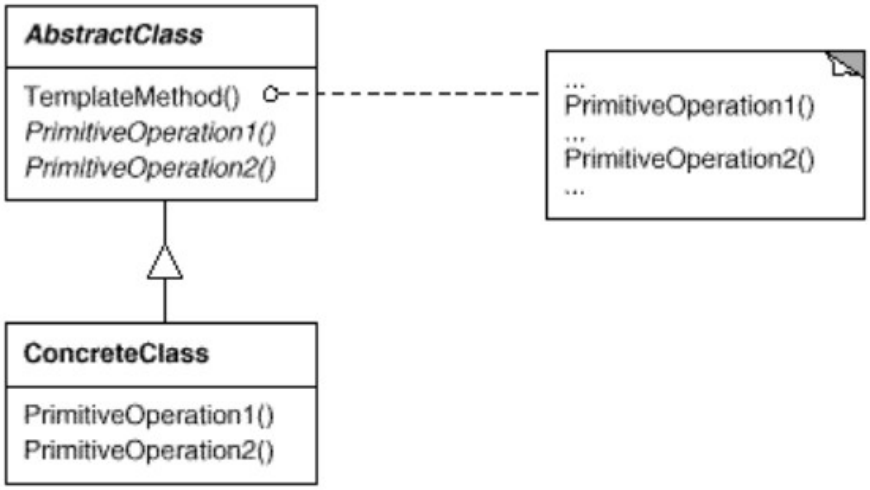
\includegraphics[width=0.4\linewidth]{../../immagini/templateMethod_Strategy/struttura_templateMethod}    
\end{figure}

\textbf{AbstractClass} 

\begin{itemize}
    \item \textit{definisce} le operazioni astratte che rappresentano i passi di un algoritmo;
    \item \textit{Implementa} il template method (l’algoritmo) che, a sua volta, chiama le operazioni astratte.
\end{itemize}

\textbf{ConcreteClass} che implementa le operazioni astratte.

\section{Strategy}

Definisce una famiglia di algoritmi, li incapsula, e li rende intercambiabili.

Lo Strategy nasconde le informazioni interne dell’implementazione di un algoritmo, una classe può avere diversi comportamenti a seconda di qualche condizione.

Prendiamo ad esempio uno Shop che può applicare più sconti, ad esempio percentuale, assoluto o nessuno sconto.

Prima di applicare lo Strategy saremo in una condizione di questo tipo
\begin{lstlisting}
public class Shop {
    private DiscountType discountType;
        public Shop(DiscountType discountType) {
        this.discountType = discountType;
    }

    public void setDiscountType(DiscountType discountType) {
        this.discountType = discountType;
    }

    public int getTotal(int originalPrice) {
        switch (discountType) {
        case NO_DISCOUNT:
            return originalPrice;
        case ABSOLUTE_DISCOUNT:
            // sottrae un valore predefinito
            // (predefinito dove?)
            return ...;
        case PERCENTAGE_DISCOUNT:
            // applica uno sconto su percentuale
            // (quale percentuale?)
            return ...;
        }
        return ...;
    }
}
\end{lstlisting}

dove il tipo di sconto può essere modificato a runtime (good) ma i dettagli interni di ogni tipo di sconto devono essere specificati nello Shop (no good) e, se 
in futuro dovessi aggiungere un nuovo tipo di sconto, dovrei mettere alla classe Shop aggiungengo un nuovo ramo all'if-else, anche se non dovrebbe essere di sua 
compentenza.

Con lo Strategy avremo 
\begin{lstlisting}
public class Shop {

private DiscountStrategy discountStrategy;
    public Shop(DiscountStrategy discountStrategy) {
        this.discountStrategy = discountStrategy;
    }

    public void setDiscountStrategy(DiscountStrategy discountStrategy) {
        this.discountStrategy = discountStrategy
    }

    public int getTotal(int originalPrice) {
        return discountStrategy.applyDiscount(originalPrice);
    }
}
\end{lstlisting}

dove il tipo di sconto può essere modificato a runtime (good) e dettagli interni di ogni tipo di sconto non riguardano Shop (good).

DiscountStrategy è la nostra interfaccia che mette a disposizione il metodo, astratto, applyDiscount(int) che sarà gestito in maniera differente in base alla tipologia
di sconto che vogliamo applicare, ad esempio
\newpage
\begin{multicols}{2}
\begin{lstlisting}
    public interface DiscountStrategy {
        int applyDiscount(int originalPrice);
    }
\end{lstlisting}
\columnbreak
\begin{lstlisting}
    public class NoDiscountStrategy implements DiscountStrategy {
        @Override
        public int applyDiscount(int originalPrice) {
            return originalPrice;
        }
    }
\end{lstlisting}
\end{multicols}

\begin{multicols}{2}
\begin{lstlisting}
    public class AbsoluteDiscountStrategy implements DiscountStrategy {
    private int discount;
    
    public AbsoluteDiscountStrategy(int discount) {
        this.discount = discount;
    }

    @Override
    public int applyDiscount(int originalPrice) {
        return originalPrice - discount;
    }
}    
\end{lstlisting}
\columnbreak
\begin{lstlisting}
    public class PercentageDiscountStrategy implements DiscountStrategy {
    private int percentage;
    
    public PercentageDiscountStrategy(int percentage) {
        this.percentage = percentage;
    }

    @Override
    public int applyDiscount(int originalPrice) {
        return originalPrice - (originalPrice * percentage / 100);
    }
}
\end{lstlisting}
\end{multicols}

\subsection{Conseguenza}

I Client devono essere consapevoli che esistono diverse strategie (cioè diverse implementazioni di una strategia).

\subsection{Struttura e partecipanti}

\begin{figure}[H]
    \centering   
    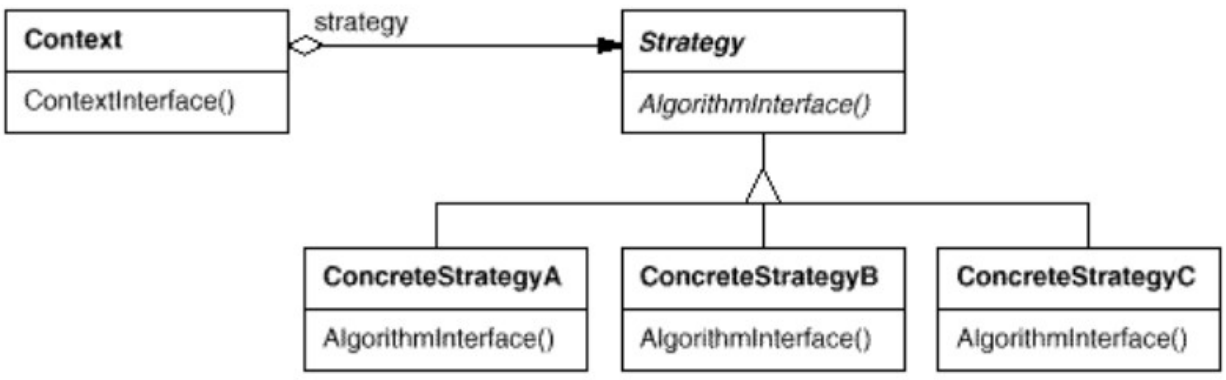
\includegraphics[width=0.5\linewidth]{../../immagini/templateMethod_Strategy/struttura_strategy}    
\end{figure}

\textbf{Strategy} dichiara l’interfaccia comune a tutti gli algoritmi supportati;

\textbf{ConcreteStrategy} implementa l’interfaccia Strategy e l’algoritmo;

\textbf{Context} usa uno Strategy quando ha bisogno dell’algoritmo che, a runtime, sarà effettivamente implementato da un ConcreteStrategy.

Context ha un riferimento a Strategy che sarà configurato assegnandogli un ConcreteStrategy passandolo al costruttore o tramite un setter, inoltre può definire a sua 
volta un’interfaccia per permettere a uno Strategy di accedere al suo stato.

\subsection{Differenza con il templateMethod}

Sembra simile al templateMethod, invece è completamente l'opposto, col templateMethod l'\textit{implementazione dell'algoritmo è fissa}, cambia solamente 
l'implementazione di alcuni suoi passi, mentre nello strategy è \textit{fisso il problema che intende risovere} l'algoritmo ma il come deve essere risolto viene 
implementato dalle sottoclassi. 

Prendiamo come esempio l'ordinamento

\begin{itemize}
    \item con il templateMethod avremo il Bubblesort come algoritmo fisso, dove al suo interno potranno \textbf{cambiare alcuni suoi passi}, quindi le sottoclassi
    estenderanno la classe Bubblesort ed implementeranno i suoi passi astratti;
    \item con lo Strartegy, si definisce un'interfaccia per l'ordinamento dove l'\textbf{algoritmo cambia}, a seconda del tipo di ordinamento,  
    (SelectionSort, InsertionSort, Bubblesort, ecc\dots..), quindi le sottoclasse implementeranno l'ordinamento desiderato e ridefiniranno l'algoritmo a proprio 
    piacimento.
\end{itemize}

Template Method sfrutta l’inheritance e l’overriding (meccanismo statico), mentre lo Strategy sfrutta l’object composition e delegation (meccanismo dinamico), 
infatti l’implementazione di strategy può essere anche modificata a runtime, ad esempio tramite il setter.

\subsection{Strategy e classi anonime}

Si può creare una classe di utilità che crea le strategy con classi anonime
\begin{lstlisting}
public class DiscountStrategies {

    //costruttore privato

    public static DiscountStrategy noDiscount() {
        return new DiscountStrategy() {
            @Override
            public int applyDiscount(int originalPrice) {
                return originalPrice;
            }
        };
    }

    public static DiscountStrategy absoluteDiscount(int discount) {
        return new DiscountStrategy() {
            @Override
            public int applyDiscount(int originalPrice) {
                return originalPrice - discount;
            }
        };
    }

    public static DiscountStrategy percentageDiscount(int percentage) {
        return new DiscountStrategy() {
            @Override
            public int applyDiscount(int originalPrice) {
                return originalPrice - (originalPrice * percentage / 100);
            }
        };
    }
}
\end{lstlisting}

\subsection{Strategy e lambda}

L’interfaccia Strategy di solito ha un singolo metodo astratto, quindi siamo in contesto lambda.
\begin{lstlisting}
public class DiscountStrategies {
    public static DiscountStrategy noDiscount() {
        return originalPrice -> originalPrice;
    }

    public static DiscountStrategy absoluteDiscount(int discount) {
        return originalPrice -> originalPrice - discount;
    }

    public static DiscountStrategy percentageDiscount(int percentage) {
        return originalPrice -> originalPrice - (originalPrice * percentage / 100);
    }
}
\end{lstlisting}

\chapter{COMPOSITE}

Pattern \underline{strutturale} (descrive la composizione di classi e oggetti), compone oggetti in strutture ad albero, adatto per tipi di dato ricorsivi.

Le classi client trattano questi oggetti in modo uniforme, indipendentemente dal fatto che si tratti di oggetti semplici o composti, inoltre non sanno e non dovrebbero
sapere se stanno interagendo con foglie o composti.

Sfrutta sia il meccanismo dell'ereditarietà e sia il meccanismo dell'object composition e delegation, il primo attraverso il fatto che un Composite è un Component, il 
secondo dove Composite è composto da tanti Component e delega operation() ai figli.

È facile aggiungere nuovi tipi di componenti, basta creare nuove sottoclassi di Leaf o di Composite.

Questi potranno essere usati immediatamente in strutture esistenti ma è difficile imporre dei vincoli sul tipo dei componenti.

Se un composto deve avere solo un certo tipo di figli, probabilmente il pattern non fa al caso nostro.

Questo pattern non può imporre vincoli statici, in quanto non possono essere controllati dal compilatore (type system) e quindi dovremmo effettuare controlli a runtime
ed eventualmente, sollevare eccezioni (no good).

Un esempio di applicazione del pattern è il FileSystem.

Avremo la classe astratta FileSystemResource (il nostro Component), la sottoclasse FileSystemFile (Leaf) e FileSystemDirectory (Composite), che contiene al suo interno
tanti oggetti di tipo FileSystemResource.

\section{Struttura}

\begin{figure}[H]
    \centering
    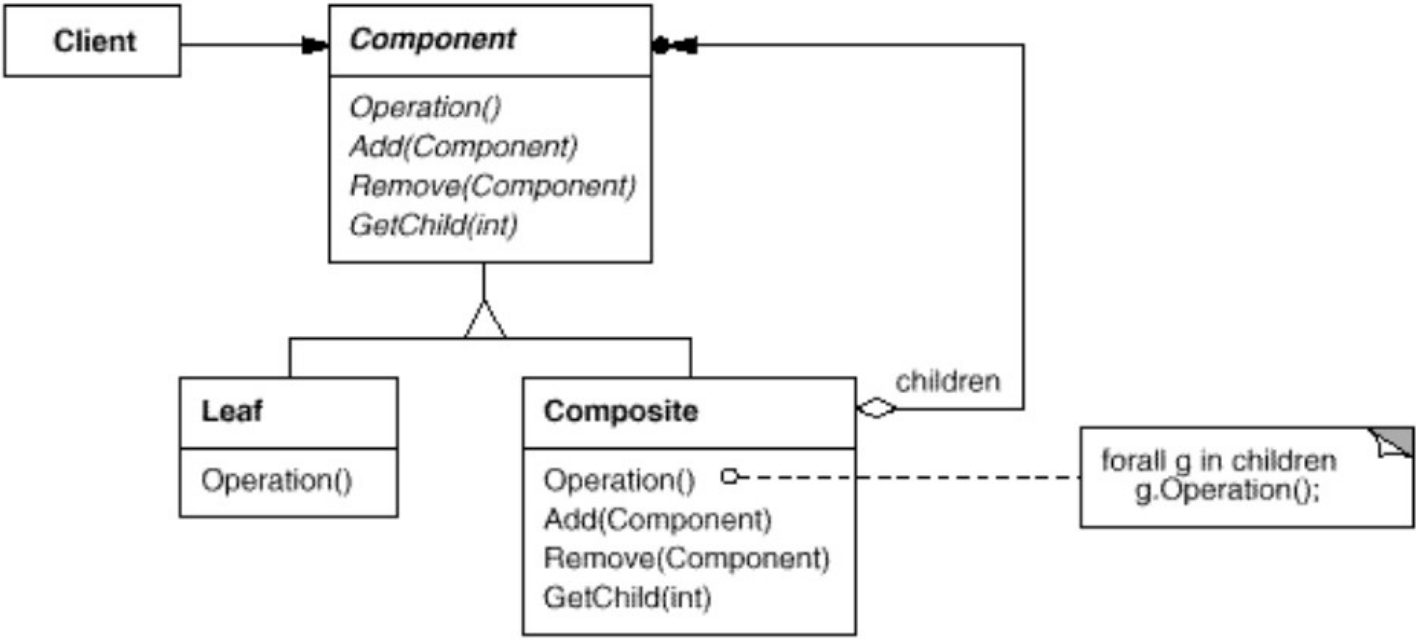
\includegraphics[width=0.5\linewidth]{../../immagini/composite/struttura_composite}
\end{figure}

\textbf{Component}
\begin{itemize}
    \item dichiara l’interfaccia comune a tutti gli oggetti della composizione;
    \item implementa il comportamento di default comune a tutte le sottoclassi, in questo caso operation();
    \item dichiara un’interfaccia per accedere a/e gestire i componenti figlio (add(), remove() e get());
    \item definisce un modo per accedere al componente padre (opzionale).
\end{itemize}

\textbf{Leaf}
\begin{itemize}
    \item rappresenta oggetti foglia della composizione;
    \item non ha figli;
    \item definisce il comportamento di default dell’interfaccia comune per gli oggetti primitivi della composizione.
\end{itemize} 

\textbf{Composite}
\begin{itemize}
    \item definisce il comportamento dell’interfaccia comune dei componenti con figli.
    \item memorizza i componenti figli;
    \item implementa le operazioni relativi alla gestione dei figli definite nell’interfaccia Component.
\end{itemize}

\textbf{Client} manipola gli oggetti della composizione attraverso l’interfaccia Component.
\medskip

Se la richiesta viene inviata ad una foglia, allora viene gestita direttamente, oppure se viene inoltrata ad un oggetto composto, allora viene inoltrata ai figli, 
facendo, eventualmente, delle operazioni prima e/o dopo l’inoltro.

Le operazioni di gestione dei figli sono in Component, quindi Leaf li dovrebbe overridare sollevando un'eccezione oppure non facendo nulla.

Per questo motivo abbiamo due versioni di questo pattern, una è quella che abbiamo visto ora, chiamata \textbf{design for uniformity}, e l'altra chiamata 
\textbf{design for tape safety} dove i metodi di gestione dei figli sono in Composite.

Nella prima i client, non sapendo se stanno trattando Leaf o Composite, potrebbero chiamare i metodi di gestione dei figli direttamente su Leaf, rischiando di 
ottenere errori a runtime.

Con l'altra versione il client non può chiamare operazioni per la gestione dei figli su Leaf, evitando così errori a runtime, può farlo solo Composite perdendo però 
uniformità.

Nella variante type safe il client dovrebbe avere un riferimento alla radice della struttura di tipo statico Composite, in caso contrario non potrebbe chiamare i 
metodi per gestire i figli.

\chapter{ITERATOR}

Pattern \underline{comportamentale}, descrivono come classi e oggetti interagiscono e si distribuiscono le responsabilità.

Usato per accedere ai contenuti di un oggetto aggregato senza esporne la rappresentazione interna e fornisce un modo uniforme per attraversarla.
\smallskip

Supponiamo di avere una classe scuola, avente una collezione privata di studenti permettendo ai client di poter aggiungere alla collezione col metodo add() e di 
volerne dare un accesso in sola lettura, attraverso un getter pubblico
\begin{lstlisting}
public class School {
    private ArrayList<Student> students = new ArrayList<>();
    
    public void addStudent(Student student) {
        students.add(student);
    }
    
    public ArrayList<Student> getStudents() {
        return students;
    }
}
\end{lstlisting}

Così facendo si espone ai client un dettaglio implementativo, ArrayList e, se un giorno decidessi di cambiare l'implementazione della collezione, i client avranno 
problemi di compilazione.

Un getter protected non migliorerebbe la situazione in quanto ai client esterni basterebbe estendere la nostra classe per usare quel getter e quindi stesso problema.
\smallskip

Utilizzando un iteratore
\begin{itemize}
    \item accediamo ai contenuti di oggetto aggregato senza esporne la rappresentazione interna;
    \item possiamo supportare diverse strategie di attraversamento;
    \item fornire un’interfaccia uniforme per attraversare strutture aggregate diverse.
\end{itemize}

\textbf{N.B.} Un iteratore non conosce il numero di elementi di un aggregato, può solamente attraversarli.
\medskip

Quindi con l'iteratore avremo
\begin{lstlisting}
public class School {
    private List<Student> students = new ArrayList<>();
    
    public void addStudent(Student student) {
        students.add(student);
    }

    public Iterator<Student> studentIterator() {
        return students.iterator();
    }
}
\end{lstlisting}

dove i client usano studentIterator() per “attraversare” sequenzialmente i vari studenti della scuola, ignorando completamente la rappresentazione interna della 
struttura che li contiene senza poter fare assunzioni sull’ordine durante l’attraversamento.

\medskip
\textbf{N.B.} Una volta usato un iteratore per un attraversamento completo, ne va usato uno nuovo.

\section{Struttura}

\begin{figure}[H]
    \centering
    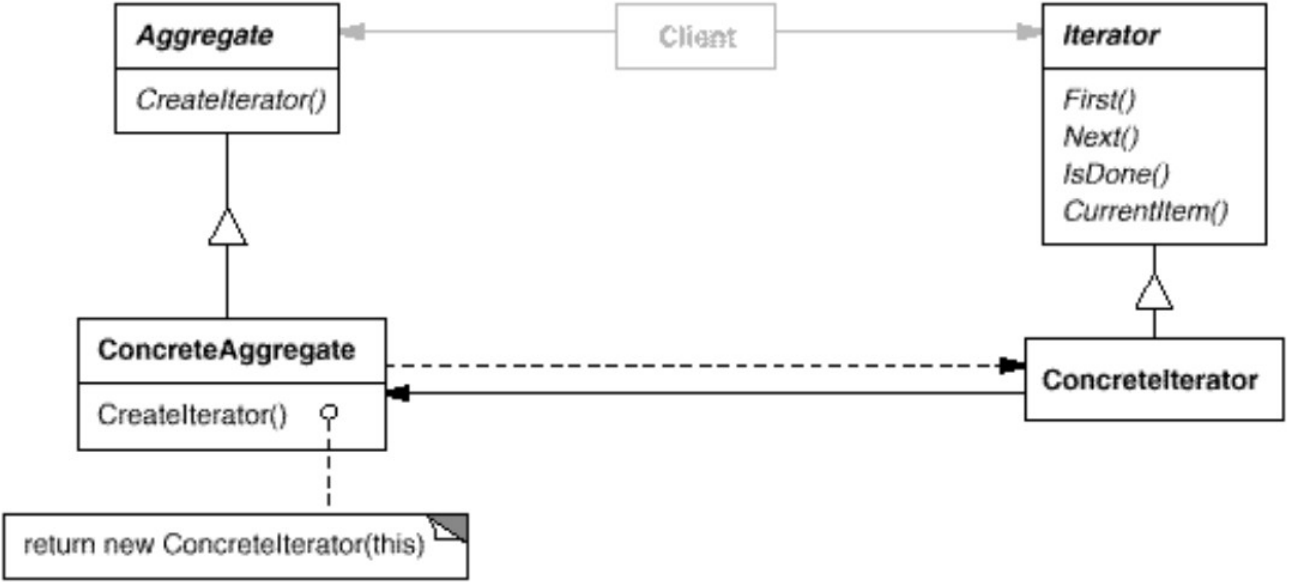
\includegraphics[width=0.5\linewidth]{../../immagini/iterator/struttura_visitor}
\end{figure}

\textbf{Iterator} definisce l'interfaccia per attraversare gli elementi e offre metodi come hasNext() per verificare se ci sono altri elementi da attraversare e next()
per ottenere l'elemento successivo;

\textbf{Aggregate} è l'interfaccia, o la classe astratta, che rappresenta la collezione di oggetti che fornisce un metodo per ottenere un iteratore che può essere 
utilizzato per attraversare gli elementi;

\textbf{ConcreteIterator} implementa Iterator, tiene traccia, durante l’attraversamento, dell’oggetto corrente, deve essere in grado di calcolare l’elemento 
successivo e ha un riferimento all’aggregato concreto;

\textbf{ConcreteAggregate} implementa Aggregate e crea un opportuno ConcreteIterator.

\section{Iterator e classi anonime}

Un iteratore concreto è tipicamente implementato come classe (privata) interna o direttamente come classe anonima, infatti deve poter accedere direttamente alla
rappresentazione interna (privata) dell’aggregato.
\begin{lstlisting}
public class School {
    private Student[] students = new Student[100];
    private int index = 0;
    
    public void addStudent(Student student) {
        // controlli per la dimensione da fare...
        students[index++] = student;
    }

    public Iterator<Student> studentIterator() {
        return new Iterator<Student>() {
            private int current = 0;

            @Override
            public boolean hasNext() {
                return current < index;
            }

            @Override
            public Student next() {
                if (current >= index)
                    throw new NoSuchElementException();
                return students[current++];
            }
        };
    }
}
\end{lstlisting}

\section{Iterator vs Stream}

Possono sembrare simili ma
\begin{itemize}
    \item gli stream sono più astratti e possono essere parallelizzati, si basano su un approccio dichiarativo, permettono facilmente di filtrare, raggruppare, 
    partizionare e \textit{gestiscono, in automatico, l’attraversamento dell’aggregato};
    \item gli iteratori sono molto più semplici, permettono di attraversare un aggregato un elemento alla volta, sono per loro stessa natura sequenziali ma 
    richiedono \textit{che hasNext() e next() siano usati correttamente insieme};
    \item creare un’implementazione di Iterator è piuttosto semplici, i metodi da implementare sono pochi;
    \item creare un’implementazione di Stream non è banale.
\end{itemize}

\chapter{PATTERN CREAZIONALI}

Questa tipologia di pattern \textit{astrae} il processo di creazione degli oggetti, fornendo diversi modi per associare un’interfaccia (o classe astratta) con 
un’implementazione e assicura che il programma sia scritto in termini di interfacce e non di implementazione.

\section{Perchè?}

Dal DIP sappiamo che è fondamentale non riferirsi a classi concrete (ma a classi astratte) e questo implica che ogni istruzione "new" mette a rischio questo principio.

Però, prima o poi, lo statement "new" deve essere usato ed è fondamentale che questo avvenga in poche e limitate parti del programma su cui abbiamo il controllo di 
flessibilità.

Se volessimo cambiare il tipo degli oggetti creati, saremmo in grado di farlo in un solo punto e senza troppe conseguenze al resto del programma.

\section{Factory Method}

Definisce un’interfaccia per creare un oggetto di un certo tipo ma lascia decidere alle sottoclassi quale oggetto istanziare.

La creazione di un'instanza avviene in un metodo (Factory method) che può essere astratto per poi essere implementato dalle sottoclassi oppure concreto per poi 
essere ridefinito dalle sottoclassi.

L'assegnazione dell'instanza viene salvata in una variabile, sempre nella classe base, privata e chi implementa/estende l'interfaccia/classe astratta avrà il compito 
di implementare/ridefinire il factory method.

Nella classe base il metodo restituirà il tipo dell'interfaccia desiderata, mentre nelle sottoclassi possiamo sfruttare la covarianza.

Nell'esempio di Application e Document, visto nel Template Method, il metodo createDocument() è il nostro factory method, infatti risulta essere astratto.

Factory Method serve a \textit{“parametrizzare”} rispetto alla creazione di un oggetto, basandosi solo su inheritance, ridefinizione di metodo e binding dinamico.

Se il linguaggio permettesse di passare un blocco di codice (lambda) che crea un oggetto, si potrebbe anche fare a meno di questo pattern ma non si parlerebbe più
di FactoryMethod.

\subsection{Struttura}
\begin{figure}[H]
    \centering
    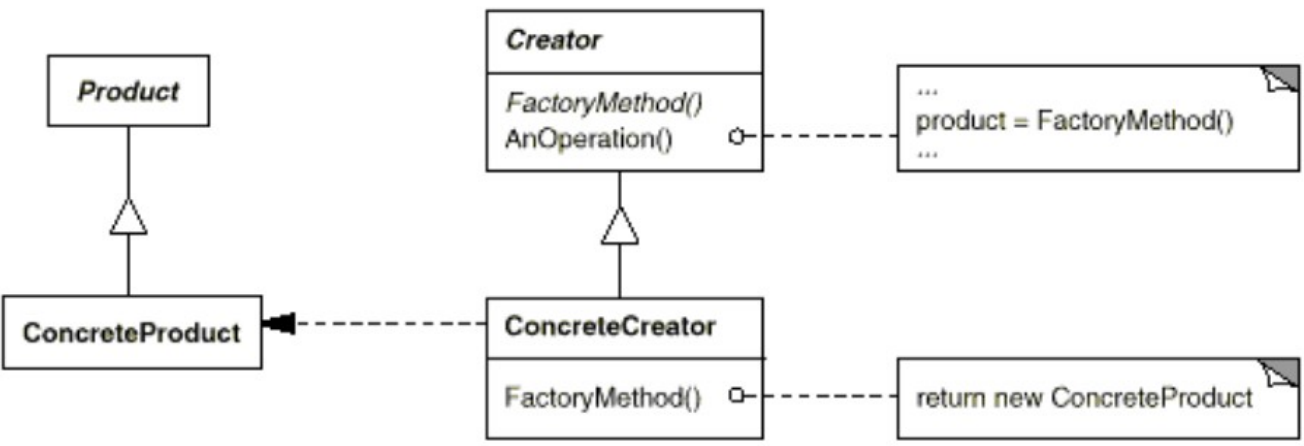
\includegraphics[width=0.5\linewidth]{pattern_creazionale/struttura_factory_method}
\end{figure}

\textbf{Product} definisce l'interfaccia degli oggetti creati tramite il FactoryMethod di Creator;

\textbf{Creator} dichiara il FactoryMethod, che restituisce un Product, con eventualmente un'implementazione di default, e lo chiama;

\textbf{ConcreteProduct} implementa l'interfaccia Product;

\textbf{ConcreteCreator} implementa o ridefinisce il FactoryMethod di Creator ritornando un ConcreteProduct.

\subsection{Factory Method vs Template Method}

Il factory method è un metodo, eventualmente \textit{astratto} e \textit{protetto}, che verrà poi implementato o ridefinito dalle sottoclassi e viene 
\textit{richiamato} da diversi metodi concreti della classe base ed è pensato per essere \textit{chiamato solo dalla classe base} (che lo dichiara).
\smallskip

Il template method è un metodo \textit{concreto}, eventualmete \textit{final}, che \textit{richiama} operazioni implementate da sottoclassi ed è pensato 
per essere \textit{chiamato dai client}

\subsection{Principale utilizzo}

Separare la creazione degli oggetti dal loro uso permette di modificare la loro creazione in modo consistente senza produrre una cascata di modifiche nel codice che 
li usa.

Molto usato nei framework, che generalmente esistono a livello astratto e non dovrebbero conoscere il tipo concreto degli oggetti da istanziare, questa responsabilità 
è lasciata al Client del framework, che provvederà a estendere il framework con sottoclassi per definire concretamente i factory methods.

Nell'esempio del Template Method, Application e Document sono la parte astratta del framework che si occupa di creare e gestire il framework, mentre la parte bassa 
è il Client che ridefinisce/implementa, a suo piacimento, i metodi.

\subsection{Vantaggi e svantaggi}

Con questo pattern si elimina la necessità di legare il codice di un’applicazione a classi concrete, il codice lavora con Product, quindi può lavorare con ogni specifico
prodotto definito dall’utente.
\smallskip

In compenso, siamo obbligati a creare una sottoclasse di Creator per creare una certa sottoclasse di Product (alternativa è quella di usare le lambda). 

Nel costruttore passiamo l'interfaccia funzionale Supplier e usiamo il suo metodo astratto, get(), nei metodi in cui assegnamo l'istanza.

Nel costruttore passiamo la lambda o sfruttiamo la method reference.

\begin{multicols}{2}
\begin{lstlisting}
public class Client {
    private MyType f;
    private Supplier<MyType> myTypeSupplier;
    
    public Client(Supplier<MyType> myTypeSupplier) {
        this.myTypeSupplier = myTypeSupplier;
    }
    public void init() {
        f = myTypeSupplier.get();
    }
    public void m() {
        f.n();
    }
    public void reset() {
        f = myTypeSupplier.get();
    }
}
\end{lstlisting}           
\columnbreak
\begin{lstlisting}
Client baseClient = new Client(MyImpl::new);
Client derivedClient = new Client(MyOtherImpl::new);
\end{lstlisting}
\end{multicols}

\section{Abstract Factory}

Fornisce un’interfaccia per creare famiglie di prodotti correlati o dipendenti senza specificare le loro classi concrete.

Il Client non crea gli oggetti direttamente ma delega la loro creazione a un altro oggetto.

\subsection{Struttura}

\begin{figure}[H]
    \centering
    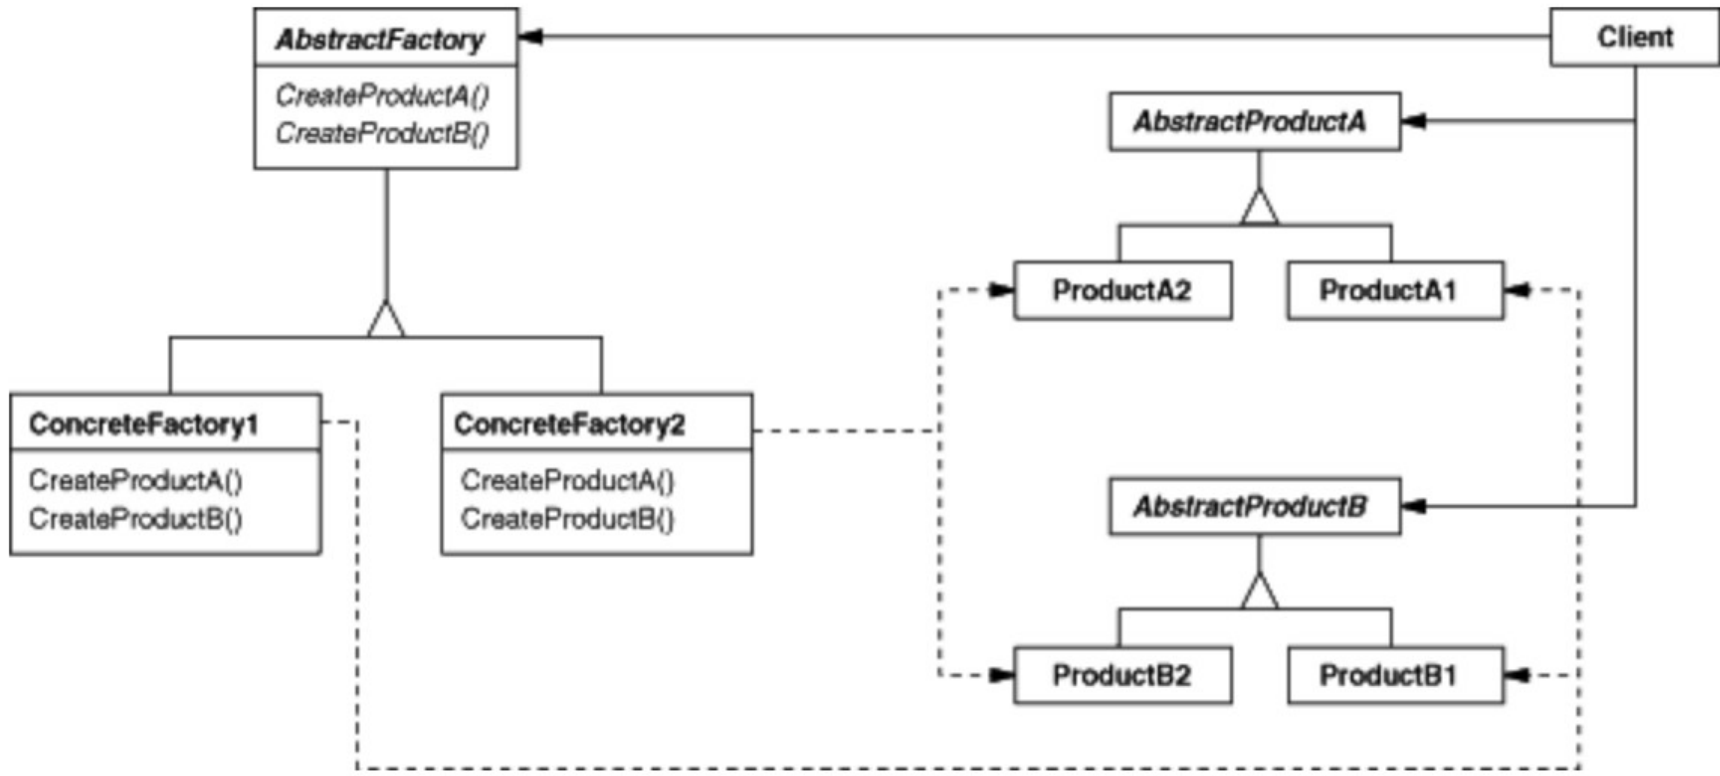
\includegraphics[width=0.5\linewidth]{pattern_creazionale/struttura_abstract_factory}
\end{figure}

\textbf{AbstractFactory} dichiara un’interfaccia per le operazioni di creazione di famiglie di AbstractProduct;

\textbf{AbstractProduct} interfaccia di una singola famiglia di prodotti;

\textbf{ConcreteFactory} implementa le operazioni per creare prodotti della stessa famiglia di un AbstractProduct;

\textbf{Product} implementazione di AbstractProduct.

\textbf{Client} utilizza l'AbstractFactory per la creazione di AbstractProduct.
\medskip

A run-time avremo una singola ConcreteFactory che crea, in modo consistente, una famiglia di prodotti.

\subsection{Conseguenze}

Se volessimo creare un'altra tipologia di prodotti, allora dovremmo istanziare ed usare un'altro tipo di ConcreteFactory, ogni famiglia di prodotti ha una propria 
implementazione di abstract factory.

Se si volesse aggiungere un nuovo prodotto, bisognerebbe aggiungere un nuovo metodo all'abstractFactory che sarà poi implementato dalle ConcretFactory.

\subsection{Principale utilizzo}

Un sistema deve essere indipendente da come gli oggetti sono creati, composti e rappresentati.

Un sistema che deve essere configurabile con una di tante famiglie di prodotti dove, i prodotti correlati di una stessa famiglia, sono progettati per essere usati 
insieme.

Si vuole fornire una libreria di oggetti rivelando solo le loro interfacce e non le loro implementazioni.

In quest'ultimo caso, le classi concrete dei prodotti, possono essere rese inaccessibili ai client mettendole in un package private, accessibili solo al package della
factory, cosicchè le factory sono le uniche a poter instanziare le classi concrete (un'altra variante è quella di usare classi anonime o interne ma avremo codice meno
leggibile).

\subsection{Accedere e modificare la factory}

Per accedere alla factory ci sono due alternative, esiste una sola instanza della factory (tramite uso del Singleton) oppure viene passata ai client attraverso un 
costruttore o setter.

Cambiare la factory a run-time può essere pericoloso in quanto, dopo il cambiamento, bisognerebbe notificare tutti i client in modo tale da ricreare tutti gli oggetti 
che sono stati instanziati attraverso la factory precedente.

Se la factory è implementata tramite Singleton, allora cambio l'instanza, se è implementata tramite setter, passo la nuova instanze oppure se è passata tramite 
costruttore, allora si ricreano le instanze dei client.

\subsection{AbstractFactory vs Factory Method}

Il primo è pensato per essere \textit{usato da altre classi} ed i suoi metodi sono \textit{pubblici}.

Il secondo è pensato per essere \textit{chiamato solo dalla classe base} (che lo dichiara) e \textit{non} deve essere pubblico.

\section{Static Factory Methods}

Sono un'alternativa alla creazione di oggetti con "new".

Dato un tipo MyType, invece di scrivere new MyType, scriveremo MyType.create dove il costruttore di MyType è reso privato e viene chiamato all'interno di un metodo 
statico di nome non necessariamente create.

A differenza dei costruttori, che sono vincolati ad avere lo stesso nome della classe e non ci possono essere più costruttori con la stessa firma, gli static factory 
method possono avere nomi più significativi.

Supponiamo di voler creare un oggetto TimeSpan specificando i secondi, minuti (entrambi interi).

Con i costruttori sarebbe più complicato perchè, anche cercando di usare l'overloading, avremo errore di compilazione in quanto avrebbero la stessa firma.

Quindi potremmo pensare di avere un unico costruttore, privato, che prende in input entrambi i parametri e creare quanti static factory method vogliamo, che ritornano
l'oggetto TimeSpan che fanno due cose differenti, uno per i secondi ed uno per i minuti.

\begin{lstlisting}
public class TimeSpan {
    private TimeSpan(int seconds, int minutes) {...}

    public static TimeSpan ofSeconds(int seconds) {
        return new TimeSpan(seconds, 0);
    }

    public static TimeSpan ofMinutes(int minutes) {
        return new TimeSpan(0, minutes);
    }
}
\end{lstlisting}

Se volessi creare un TimeSpan con le ore, basterebbe modificare il costruttore senza problemi, perchè privato, aggiungere le ore, creare un nuovo static factory method, 
chiamare al suo interno il nuovo costruttore e aggiornare gli static factory method esistenti.

\medskip
\textbf{N.B.} Se il construttore fosse stato pubblico, allora, dopo l'aggiunta del terzo parametro, avremmo avuto problemi di compilazione sia sul nostro codice che su 
quello dei client esterni.
\medskip

Quando si invoca un costruttore (tramite un "new") viene sempre creato un nuovo oggetto, con gli static factory methods, invece, si possono restituire oggetti condivisi.

\section{Singleton}

Assicurare che una classe abbia una sola istanza e ne fornisce un punto di accesso globale.

Viene implementato tramite uno static factory method (per convenzione si chiama getInstance) che restirtuisce l'instanzia in un campo statico privato 
(eventualmente crea l'oggetto la prima volta che viene chiamato).

\begin{lstlisting}
public class MyClass {
    private static MyClass instance = null;
    
    private MyClass() {...}

    public static MyClass getInstance() {
    if (instance == null) {
        instance = new MyClass();
    }
        return instance;
    }
}
\end{lstlisting}

\section{Fluent Interface}

Questo design pattern si basa sul Method Chaining, ovvero ogni metodo ritorna un oggetto, in modo da concatenare insieme tante invocazioni in un singolo statement, 
senza dover salvare i risultati intermedi in variabili locali.

Viene usato per fare il design delle API Object-Oriented, quindi tipico delle librerie e dei framework.

Un tipico caso d’uso è rimpiazzare i setter per rendere la configurazione di un oggetto più facile.

\section{Builder}

Separa la costruzione di un oggetto complesso dalla sua rappresentazione, la configurazione non viene fatta nel costruttore ma viene gestita da un altro oggetto, 
il builder (si basa su fluent interface).

La costruzione viene preparata passo-passo e infine viene effettivamente creata l’instanza.

La classe builder è una static inner class della classe di cui si vogliono costruire oggetti, il costruttore prende gli argomenti per i campi “richiesti” 
(non opzionali), fornisce metodi per specificare argomenti per campi opzionali, che non vengono applicati subito ai campi dell’oggetto da creare ed infine fornisce un 
metodo, build(), che crea effettivamente l’oggetto usando gli argomenti raccolti per i vari campi.

La classe di cui si vuole costruire l'oggetto ha il costruttore e setter privati, in questo modo solo la classe builder vi può accedere e diventa l’unico modo per 
istanziare oggetti della classe.

L’oggetto, una volta costruito, è sempre valido, eventuali problemi negli argomenti passati vengono rilevati durante la creazione del builder e non dopo.

Supponiamo di avere una classe Person che ha dei campi che deve avere obbligatoriamente ed altri opzionali.

Per applicare il pattern, il costruttore di Person deve essere privato.

\begin{lstlisting}
public class Person {
    private int id; // richiesto
    private String name; // richiesto

    private Integer age; // opzionale con validazione
    private String address; // opzionale senza validazione

    // costruttore privato ed, eventualmente, getter pubblici
}
\end{lstlisting}

Aggiungiamo la classe builder, che è una static inner class che ha gli stessi parametri della classe ospitante.

\begin{lstlisting}
public class Person {
    ...
    public static class PersonBuilder {
        private int id;
        private String name;
        private Integer age;
        private String address;
        
        public PersonBuilder(int id, String name) {
            this.id = id;
            this.name = name;
        }
        ...
    }
    ...
}    
\end{lstlisting}

Aggiungiamo anche i metodi per i campi opzionali (ritorano sempre un builder) e, per convenzione, cominciano con with (non hanno nulla in comune con i withers
che invece resituiscono una copia dell'oggetto con qualcosa di diverso).

\begin{lstlisting}
public class Person {
    ...
    public static class PersonBuilder {
        
        //dichiarazione dei parametri
        
        //costruttore dei parametri obbligatori
        
        public PersonBuilder withAge(Integer age) {
            if (age <= 0)
                throw new IllegalArgumentException("age must be positive: " + age);
            this.age = age;
            return this;
        }
        public PersonBuilder withAddress(String address) {
            this.address = address;
            return this;
        }
    }
    ...
}       
\end{lstlisting}

Infine il metodo build che costruisce l’oggetto e che ritorna il tipo della classe ospitante.

\begin{lstlisting}
public class Person {
    ...
    public static class PersonBuilder {
        
        //dichiarazione dei parametri
        
        //costruttore dei parametri obbligatori
        
        //metodi per i parametri opzionali

        public Person build() {
            Person person = new Person();
            person.setId(id);
            person.setName(name);
            person.setAge(age);
            person.setAddress(address);
            return person;
        }
    }
    ...
} 
\end{lstlisting}

Per creare un oggetto Person, bisognerà accerdere prima al costruttore del builder, chiamare i metodo opzionali ed infine usare il metodo build 
(sembra uno stream, infatti anche loro si basano su fluent interface).

Se il build va a termine, significa che l'oggetto creato è valido, in caso contrario avremo errori prima della sua effettva creazione (vedi il metodo withAge).

\begin{lstlisting}
Person person = new Person.PersonBuilder(1, "John")
                            .withAge(10)
                            .withAddress("an address")
                            .build();
\end{lstlisting}


\chapter{OBSERVER}

E' un design pattern comportamentale utilizzato per gestire le relazioni uno a molti quando lo stato di uno degli oggetti cambia e si richiede l'aggiornamento automatico di 
altri oggetti dipendenti.
\medskip

Classico esempio è quello di excel dove abbiamo una cella caratterizzata da una formula che fa riferimento a più celle "satellite" ed ogni volta che modifichiamo il
valore di questi satelliti, la cella caratterizzata dalla formula cambia di conseguenza.
\medskip

Questo pattern è basato sul concetto di un oggetto (\textbf{subject}) che tiene traccia dei suoi osservatori (\textbf{observers}).

Tutti gli observer vengono notificati ogni volta che il subject cambia il suo stato (è il subject che notifica e non sono gli osservatori che controllano ogni tot tempo).

A quel punto ogni observer può ispezionare lo stato del subject e aggiornare il proprio stato.

\medskip
\textbf{Il subject non conosce quali observer lo osservano, lui si mantiene una lista di observer ma non conosce la loro implementazione concreta 
(\textbf{accoppiamento astratto} o abstract coupling).
Quando notifca, lui non sa a chi sta veramente notificando.}
\medskip

Questo pattern favorisce la riduzione della dipendenza tra il soggetto e gli osservatori, permettendo di aggiungere o rimuovere osservatori senza modificare il 
soggetto stesso. 

Inoltre, favorisce un design flessibile e scalabile, permettendo di gestire in modo efficiente le relazioni tra gli oggetti in un sistema software.

\section{Struttura}

\begin{figure}[h]
    \centering
    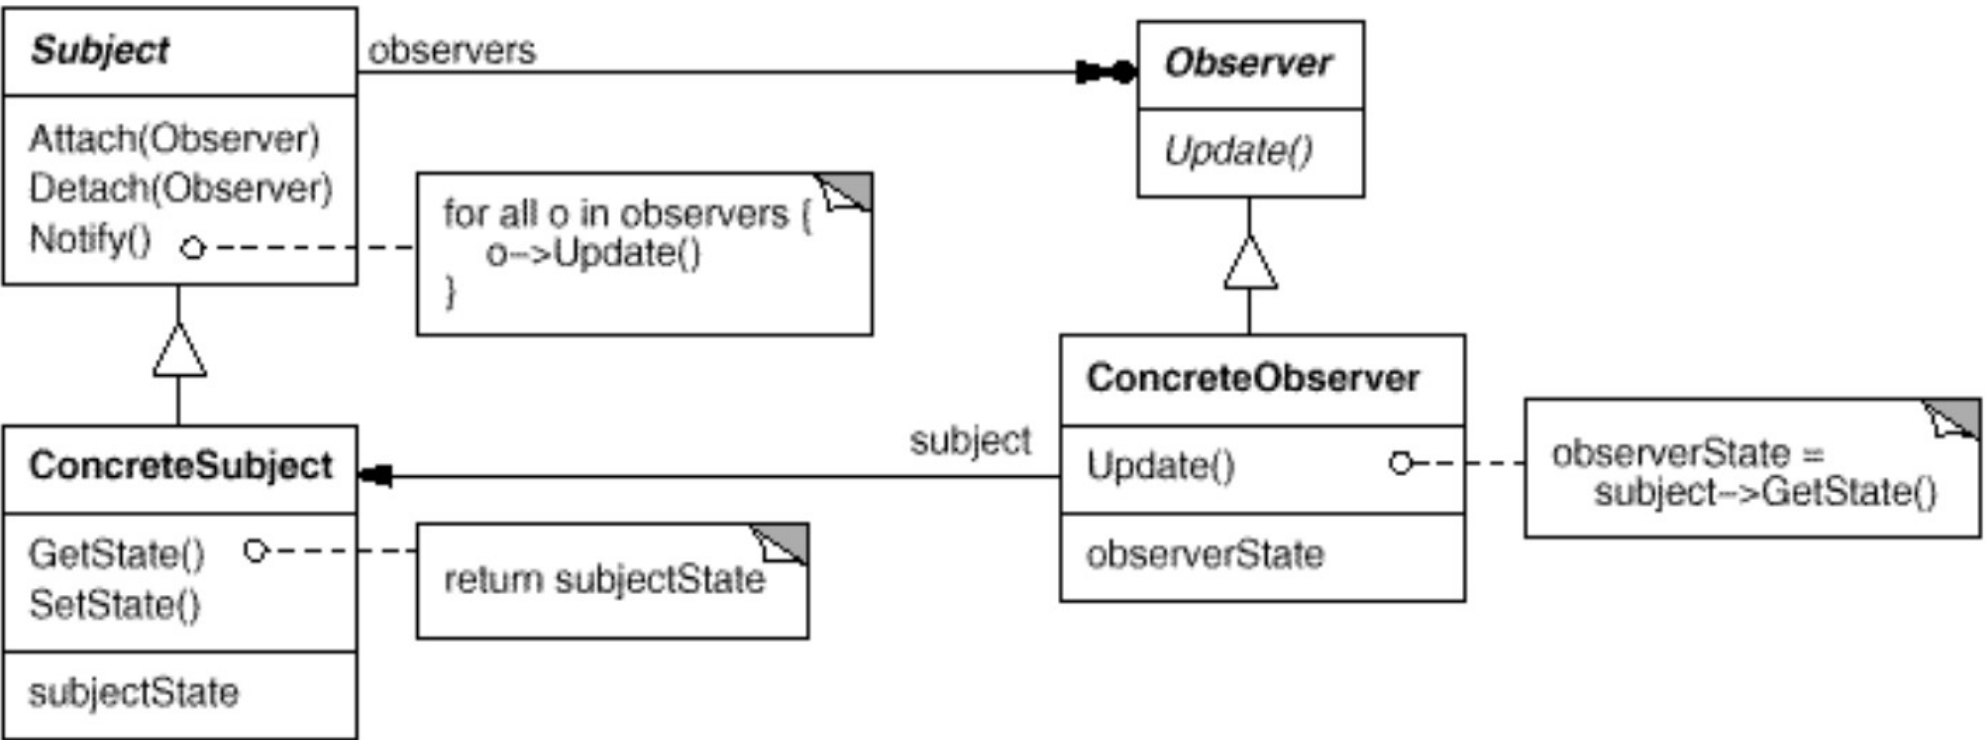
\includegraphics[width=0.5\linewidth]{../../immagini/observer_publishSubscribe/struttura_observer}
\end{figure}

\textbf{Subject} fornisce un'interfaccia per aggiungere, rimuovere e notificare gli Observer, ne conosce solamente l'interfaccia e può essere osservato da qualsiasi 
Observer.

\textbf{Observer} definisce l'interfaccia per gli oggetti che devono essere notificati riguardo il cambiamento del Subject.

\textbf{ConcreteSubject} mantiene uno stato da fornire ai ConcreteObserver.

\textbf{ConcreteObserver} ha un riferimento a ConcreteSubject ed un proprio stato che deve essere consistente al ConcreteSubject. 

\section{Interazione}

ConcreteSubject notifica i suoi osservatori quando avviene un cambiamento che potrebbe rendere lo stato degli Observer inconsistente col proprio.

Durante la notifica il ConcreteObserver può ispezionare il Subject per ottenere le informazioni per aggiornare il proprio stato, in modo da renderlo consistente con
quello del Subject.

\section{Conseguenze}

Observer non si riferisce a Subject ma è Subject che si riferisce agli Observer notificandoli.

ConcreteObserver ha un riferimento diretto a ConcreteSubject, mentre ConcreteSubject non lo ha, lo fa indirettamente chiamando il metodo di notifica ereditato da Subject.

Il Subject invia una notifica, in modalità broadcast a tutti i suoi Observer e spetterà all'Observer capire se la notifica è di suo interesse oppure no.

\section{Notifica}

Se la notifica parte dal Subject, allora i client non sono responsabili della notifica ma se il client cambia in sequenza più campi dello stesso Subject, allora 
avremo numerose notifiche consecutive (inefficienza).

Se la notifica viene chiamata dal client, ad esempio dopo vari cambiamenti chiama la notifica, è lui il responsabile della chiamata ma almeno si evitano le numerose 
notifche continue (sperando che il client si ricordi di chiamare la notifca).

\section{Svantaggio}

Il pattern è sincrono, ovvero, durante la notifica, aspetta che tutti i suoi Observer aggiornino il proprio stato.

Uno di questi Observer potrebbe essere maldestro, nel senso che ci mette troppo tempo, bloccando tutti gli altri Observer, oppure maligno, magari lanciando un'eccezione.

\chapter{PUBLISH SUBSCRIBER}

Pattern basato su messaggi, abbiamo un Publisher che invia il messaggio ed un Subscriber che si sottoscrve ad un certo tipo di messaggio.

\section{Publish subscribe vs Observer}

I Publisher non inviano direttamente il messaggio ai Subscriber (mentre nel Observer è prorpio così) ma sono affidati ad un intermediario (\textbf{broker}) che si 
occupa di consegnare il messaggio al Subscriber appropriato (nell'Observer sono loro a decidere se è di loro interesse o meno).

Quindi Publisher e Subscriber sono completamente scorrelati (mentre nel Observer abbiamo una specie di accoppiamento astratto).

Questo pattern è asincrono (mentre l'altro è l'opposto), ovvero una volta che il Publisher consegna il messaggio al broker, lui continua a svolgere i propri compiti 
ed i mesaggi saranno consegnati, non subito, ai Subscriber appropriati (thread paralleli) ed è alla base dei sistemi ad evento (java swing) dove il messaggio è l'evento 
e i subscribe sono chiamati listener che si registrano e rimangono in ascolto di un determinato evento.

\section{Vantaggio}

Questo pattern permette di avere un filtraggio dei messaggi, i subscriber dichiarano interesse per un certo tipo di messaggio e il broker si occuperà di consegnare ai 
subscriber solo i messaggi appropriati.

\chapter{DECORATOR}

Pattern \underline{strutturale}, ovvero descrive come classi e oggetti vengono composti per formare strutture più ampie. 

E' basato su object composition e delegation e il suo intento è quello di aggiungere, dinamicamente, responsabilità ad un oggetto senza influenzare altri oggetti.
\smallskip

L'idea di base è quella di racchiudere l'oggetto (\textbf{decorato}) in un altro oggetto (\textbf{decoratore}) che delega i metodi all'oggetto decorato aggiungendo del 
comportamento prima o dopo la inoltro.

Il decoratore ha la stessa interfaccia dell’oggetto decorato, quindi la sua presenza è trasparente per i client e ciò permette di avere tanti decoratori annidati
ricorsivamente.
\section{Struttura}

\begin{figure}[H]
    \centering
    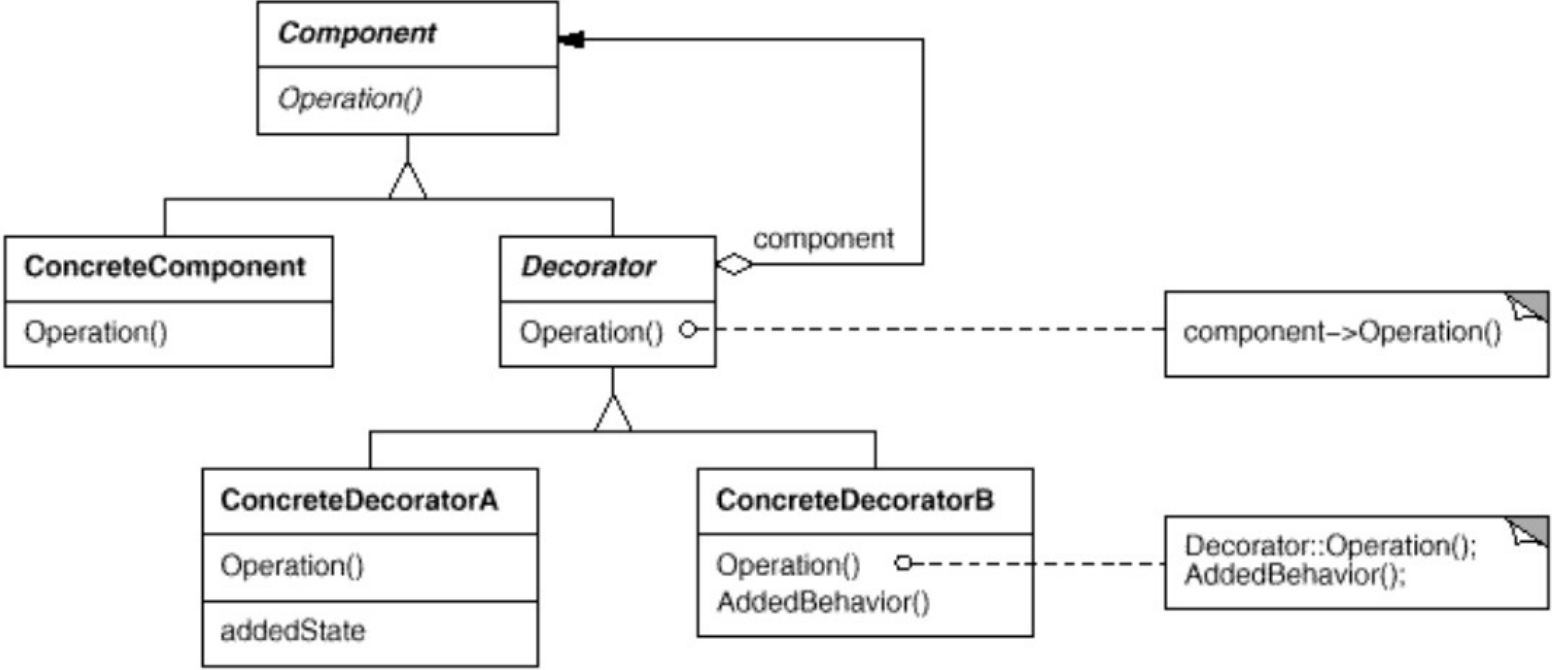
\includegraphics[width=0.5\linewidth]{decorator/struttura_decorator}    
\end{figure}

\textbf{Component} definisce l'interfaccia per gli oggetti a cui è possibile aggiungere, dinamicamente, nuove responsabilità;

\textbf{ConcreteComponent} implementa Component;

\textbf{Decorator} ha un riferimento a un oggetto Component e definisce un'interfaccia conforme a Component;

\textbf{ConcreteDecorator} aggiunge responsabilità all'oggetto Component.
\medskip

Il Decorator inoltra, di default, le richieste al suo oggetto Component e i ConcreteDecorator aggiungono il comportamento prima o dopo l'inoltro.

\medskip
\textbf{N.B.}L'inoltro ci deve sempre essere, altrimenti rompiamo la catena di decorazione.
\medskip

Per l’interface conformance, decorator e ConcreteComponent devono avere una superclasse comune e tale interfaccia, Component, deve essere il più leggera possibile, 
deve concentrarsi solo sul definire un'interfaccia e non uno stato in quanto mettere troppe funzionalità in Component porterà, le sottoclassi, ad avere funzionalità 
che non gli competono.

\section{Conseguenza}

Il pattern Decorator fornisce un modo più flessibile per aggiungere responsabilità rispetto all’inheritance
\begin{itemize}
    \item coi decorator si aggiungono responsabilità a runtime aggiungendo decorator;
    \item con l’inheritance invece si avrebbe un’esplosione delle classi.
\end{itemize}

Un sistema basato su questo pattern avrà a che fare con tanti piccoli oggetti che differiscono per il modo in cui sono iterconnessi e composti.

Questi sistemi sono flessibili e facili da customizzare ma sono difficli da comprendere e debuggare.

Uno stesso oggetto Decorator non può essere usato per decorare due componenti, potremmo cambiare il componente da decorare se aggiungiamo un setter nel decorator ma 
lo stesso oggetto decoratore può decorare sempre un solo componente alla volta.

\section{Decorator vs Strategy}

Il Decorator rispetta il principio \textit{"Changing the skin of an object versus changing its guts"} (cambiare la pelle invece delle viscere), cambia la pelle di un 
oggetto avvolgendolo in un decoratore, invece lo Strategy cambia le viscere, ovvero l'oggetto delega allo Strategy il comportamento da seguire.
\smallskip

Component non è a conoscenza dei suoi decoratori, il client utilizza, \textit{senza saperlo}, il Decorator più esterno che farà qualcosa prima o dopo l'inoltro al 
Component che, a sua volta, se sarà un altro decoratore farà la stessa cosa, altrimenti applicherà il comportamento di default.

Nello Strategy, il client \textit{è consapevole} delle diverse implementazioni (ha un riferimento allo Strategy).
\smallskip

Il Decorator ha la stessa interfaccia del suo Component mentre lo Strategy ha la sua interfaccia con diverse implementazioni concrete.

\section{Implementazione senza e con l'entità AbstractDecorator}

Sono due versione del pattern Decorator, nella prima avremo l'interfaccia SaySomething implementata direttamente sia da SaySomethingConcrete che da 
SaySomethingBeforeConcreteDecorator e SaySomethingAfterConcreteDecorator dove i due decoratori avranno un riferimento a SaySomething e chiameranno direttamente 
l'inoltro su quest'ultimo, aggiungendo del comportamento prima o dopo l'effettivo inoltro.

Nella seconda versione, SaySomething verrà implementata da SaySomethingConcrete e da SaySomethingDecorator che verrà estesa dai decoratori visti prima.

A differenza della prima versione, sarà SaySomethingDecorator ad avere un riferimento a SaySomething e ci chiamerà l'inoltro, mentre i due decoratori si occuperanno di 
aggiungere del comportamento prima o dopo l'inoltro, inoltre, non avendo un riferimento diretto a SaySomething, non potranno chiamare l'inoltro su SaySomething, ma lo 
delegheranno a SaySomethingDecorator attraverso il super.

\begin{figure}[H]
\begin{minipage}[c]{9cm}
    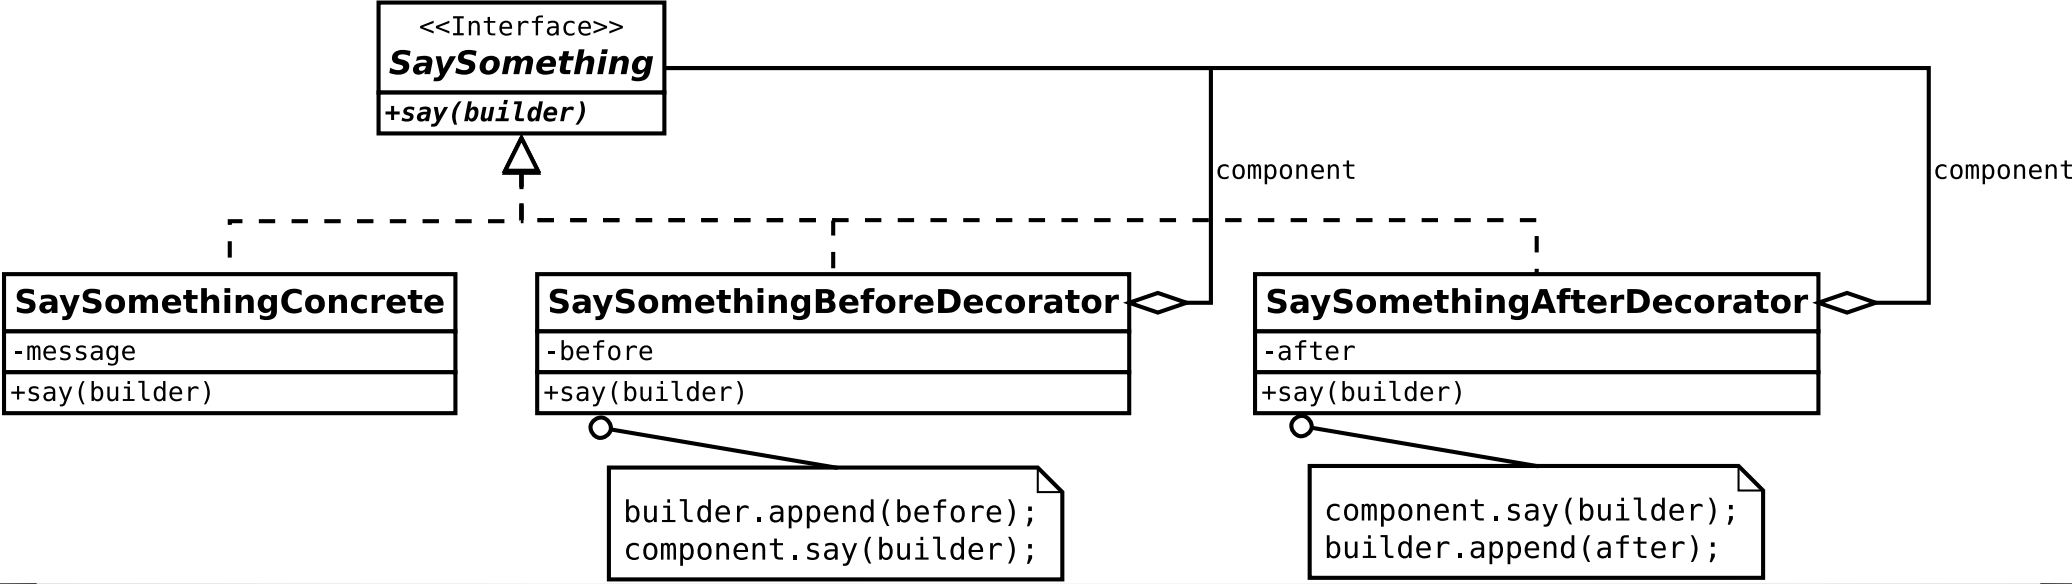
\includegraphics[width=1\linewidth]{decorator/senza_AbstractDecorator}
\end{minipage}
\hfill
\begin{minipage}[c]{8cm}
    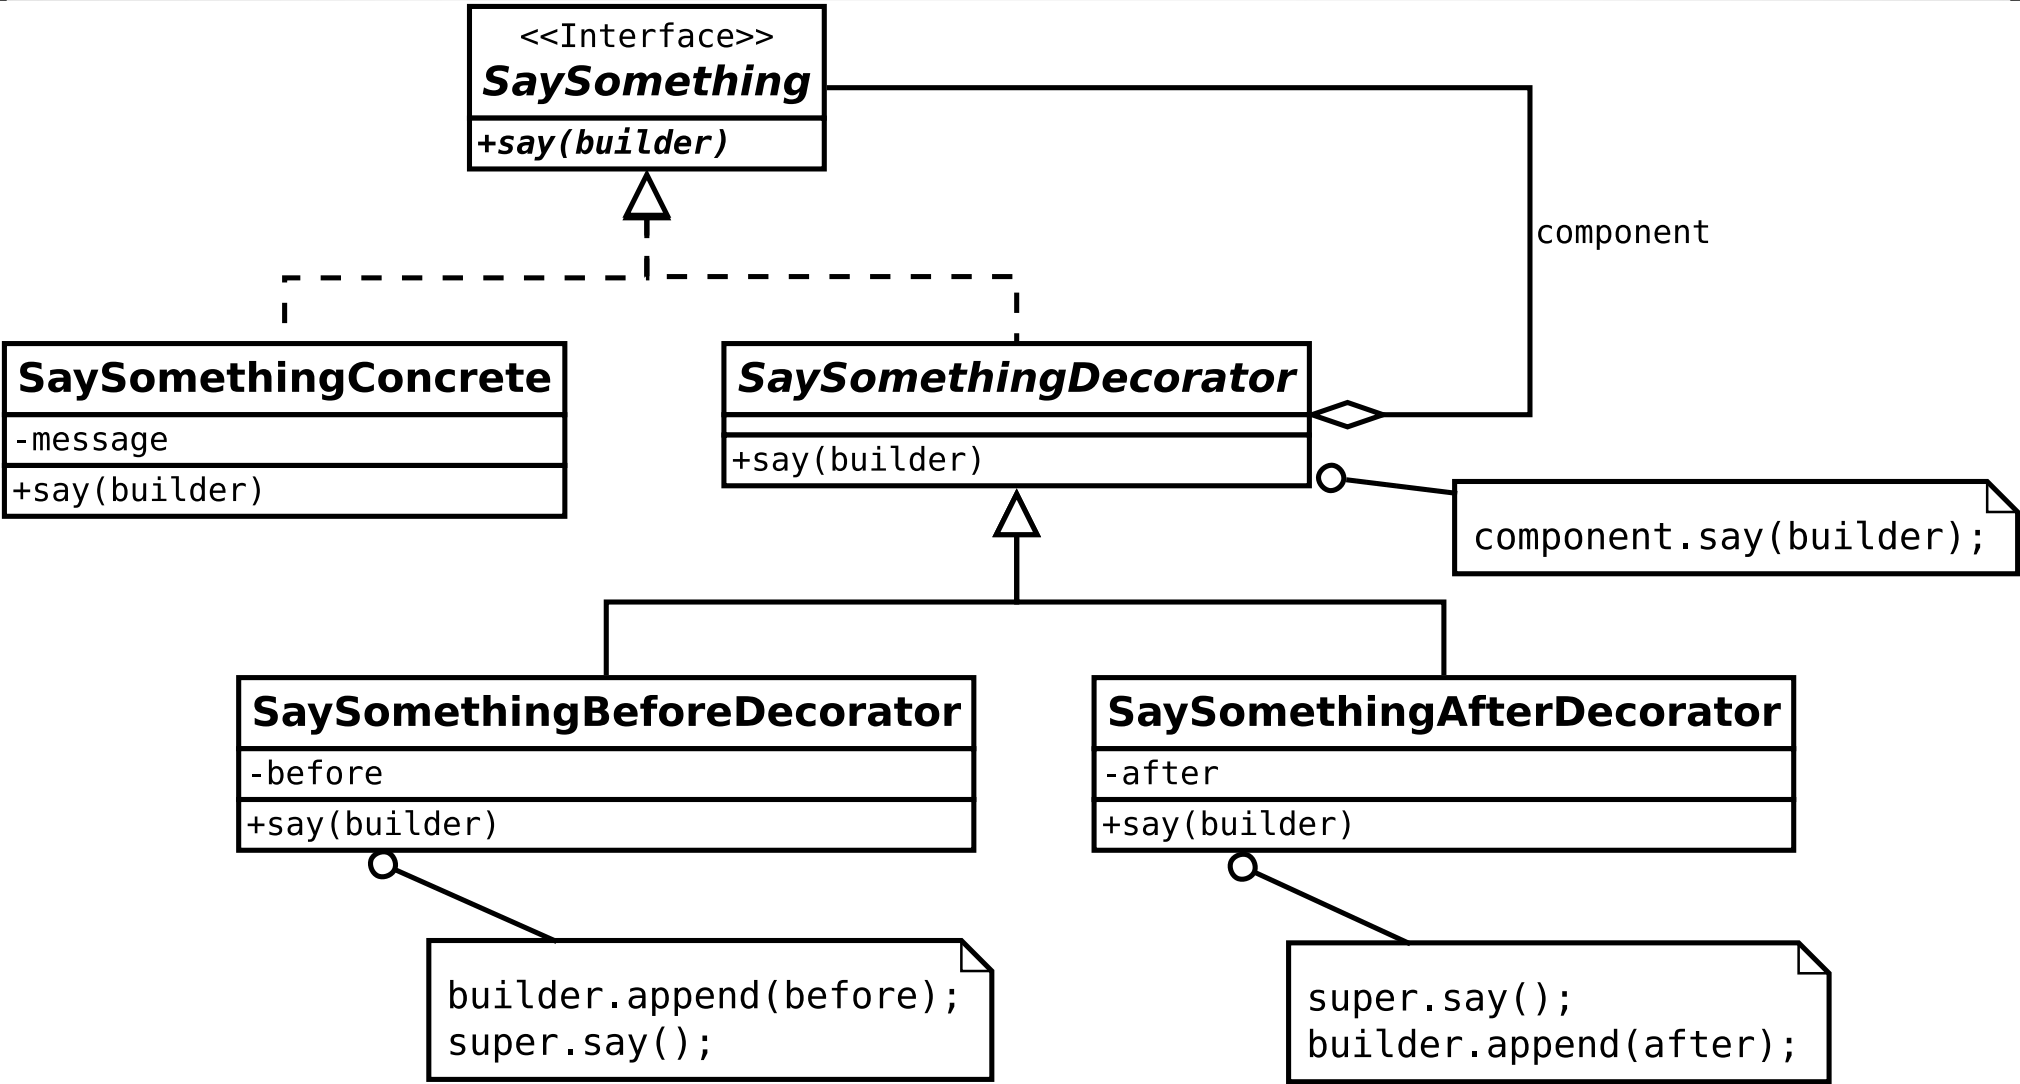
\includegraphics[width=1\linewidth]{decorator/con_AbstractDecorator}
\end{minipage}
\end{figure}

Aggiungere nuovi tipi di decorator è facile, basta implementare/estendere e poi avvolgere SaySomething.

Il difficile è rimuovere un decorator in quanto la catena delle decorazioni deve essere ricreta, dove l'oggetto SaySomething finale non deve essere re-istanziato, 
mentre i decoratori intermedi si.
\medskip

\textbf{N.B.} Quando passiamo il componente da decorare in un decorator, il componente non deve essere null (deve essere documentato nel javadoc), infatti occorre 
fare un controllo la prima volta che ci viene fornito un componente da decorare null (bisognerà anche testare questo scenario).

\section{L'inoltro}

In questo pattern potrebbe capitare di dimenticarsi di inoltrare al Component (non deve succedere).

Per evitare ciò, potremmo rendere il metodo di inoltro, nella classe Decorator, final, e di definire due metodi, astratti, che aggiungono del cambiamento prima e dopo 
l'inoltro.

In questo modo le sottoclassi non potranno dimenticarsi di inoltrare al componente, anche perchè non possono ridefinirlo essendo final, ma avranno il compito di 
implementare i metodi astratti definiti in Decorator.

Il fatto rendere il metodo final e lasciare alcuni suoi passi astratti è un esempio di template method, molti pattern sono usati insieme.

\section{Lambda}

Il pattern Decorator sfrutta il meccanismo dell'ereditarietà, object composition e delegation per sopperire alla mancanza della composizione di funzioni.

Se il linguaggio supporta le lambda, allora, invece di usare i tre meccanismi, possiamo usarle per avere lo stesso risultato ma, a quel punto, non parliamo più di 
Decorator.

Le lambda si usano con le interfacce funzionali (un solo metodo), quindi è applicabile solo al Component che ha uno ed un solo metodo da decorare.

Quindi, nell'esempio visto prima, SaySomething è un'interfaccia funzionale, quindi eleggibile all'utilizzo delle lambda.

Una stessa lambda può essere usata più volte all'interno di una composizione (invece con i decorator dovevamo creare obbligatoriamente due instanze per la stessa 
funzione), inoltre la composizione di una lambda è \textit{lineare} (fluent interface), mentre la composizione del Decorator è \textit{annidata} (la linearità è 
più leggibile).

\chapter{CHAIN OF RESPONSABILITY}

Pattern \underline{comportamentale} avente lo scopo di evitare di associare il mittente di una richiesta al suo destinatario, dando a più di un oggetto la 
possibilità di gestire la richiesta.

Il primo oggetto della catena che riceve la richiesta, la gestisce oppure la inoltra al prossimo candidato che si comporterà nello stesso modo. 

Il client che effettuerà la richiesta, non dovrà preoccuparsi di chi dovrà gestirla, anche perchè non sa chi la gestirà, quindi è fondamentale che gli oggetti 
della catena abbiamo la stessa interfaccia.

\section{Applicabilità}

Quando più oggetti possono gestire una richiesta ma non è noto a priori chi lo farà oppure il caso in cui l’insieme di oggetti che possono gestire una richiesta devono 
essere specificati dinamicamente.

\section{Struttura}

\begin{figure}[H]
    \centering
    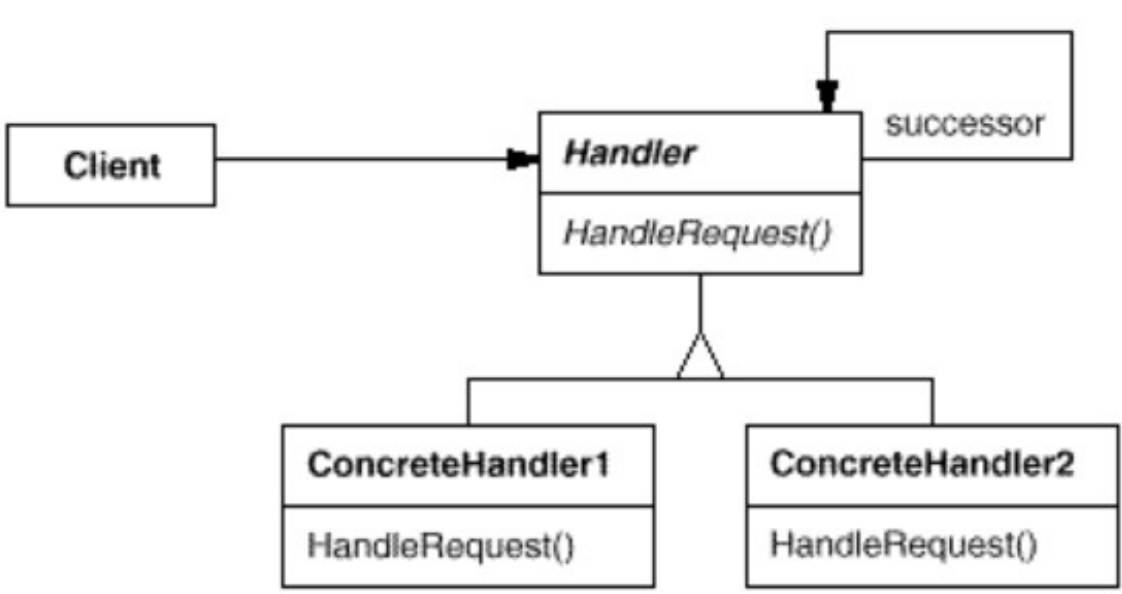
\includegraphics[width=0.4\linewidth]{../../immagini/chain_of_responsability/struttura_handler}
\end{figure}

\textbf{Handler} definisce l'interfaccia per gestire le richieste ed eventualmente implementa il riferimento al successore nella catena;

\textbf{ConcreteHandler} gestisce le richieste per cui è responsabile, può accedere al successore e se può gestire la richiesta, lo fa, altrimenti la inoltra al 
successore;

\textbf{Client} invia la richiesta chiamando un metodo sul primo elemento della catena, ignorandone il tipo effettivo.

Il successore di un Handler può essere passato direttamente al costruttore oppure tramite un setter.

Nel primo caso, dopo che abbiamo creato la catena, non la possiamo più modificare, mentre nel secondo caso è consentito stando però attenti al non creare cicli.

\section{Conseguenze}

\textbf{Reduce coupling}, Client e ConcreteHandler sono scollegati, liberiamo il Client dal dover sapere (e non deve sapere) chi gestirà la sua richiesta. 

Un oggetto della catena non conosce la struttura della stessa ma conosce solamente il suo successore.

\textbf{Maggiore flessibilità nell'assegnazione delle responsabilità agli oggetti} dove la catena viene costruita a run-time e le responsabilità possono essere 
aggiunte o rimosse modificando la stessa.

\textbf{Ricezione non garantita}, ovvero, siccome la richiesta non ha un gestore esplicito, non c'è garanzia che venga gestita (la richiesta scorre tutta la catena).

\section{L'inoltro}

Come nel Decorator, per evitare di dimenticarsi l'inoltro, possiamo definire la logica dell'inoltro nella classe base (metodo final), chiamare al suo interno un metodo 
astratto, che conterrà la logica della gestione della richiesta che sarà poi implementata dalle sottoclassi.

\section{Decorator vs Chain of responsability}

Entrambi i pattern sembrano simili ma 

\begin{multicols}{2}
    \begin{itemize}
        \item [] ha due classi principali astratta;
        \item [] \textit{tutte} le classi gestiscono la richiesta;
        \item [] il componente da decorare non deve essere null;
        \item [] pattern strutturale
    \end{itemize}
\columnbreak
    \begin{itemize}
        \item [] ha una classe astratta;
        \item [] la richiesta sarà gestita da \textit{una ed una sola} classe oppure non viene gestita;
        \item [] l'ultimo componente della catena è null;
        \item [] pattern comportamentale
    \end{itemize}
\end{multicols}

\section{Lambda}

Come il Decorator, anche questo pattern simula la composizione di funzioni.

Quindi possiamo pensare di usare una lista di lambda, scorriamo questa lista che potrà terminare perchè troveremo una lambda che riesce a gestire la richiesta oppure 
perchè lista si esaurisce in quanto non abbiamo una lambda in grado di gestire la richiesta.

Però non stiamo più parlando del pattern Chain of Responsability.


\chapter{Visitor}

E' un pattern \underline{comportamentale}, descrive come classi e oggetti interagiscono e si distribuiscono le responsabilità. 
\smallskip

Consente di definire una nuova operazione senza modificare le classi degli oggetti su cui opera ed è utile quando si ha una gerarchia di classi e si desidera eseguire 
diverse operazioni su di esse senza dover aggiungere nuovi metodi a ciascuna classe (le operazioni variano a seconda del tipo di classe concreta).

\section{Funzionamento}

Avremo un'interfaccia comune, AbstractVisitor, che definisce metodi del tipo visitXXX per ogni tipo \underline{concreto} della struttura e le sottoclassi concrete che 
estendono AbstractVisitor.

Nella classe base/interfaccia della gerarchia aggiungiamo il metodo accept(...) che prende in input un AbstractVisitor e le classi concrete della gerarchia 
implementeranno tale metodo chiamando il corrispettivo metodo visitXXX passando se stesso come input.
\medskip

\textbf{N.B.} Questo pattern sopperisce alla mancanza del \underline{double dispatch}  (overloading dinamico).
\medskip

Supponiamo di prendere in considerazione l'esempio dell'esercitazione Expression.

Quindi avremo la nostra interfaccia ExpressionVisitor con due metodi, visitConstant e visitSum che prendono in input, rispettivamente, un Constant ed un Sum e una sua 
implementazione concreta, ParenthesisRepresentationVisitor. 

Nell'interfaccia Expression avremo il metodo accept(...) che prende in input ExpressionVisitor ed infine avremo le classi Constant e Sum che implementeranno accept(...) 
chiamando rispettivamente visitConstant e visitSum.

\section{Double dispatch}

Supponiamo di avere il seguente test

\begin{lstlisting}
@Test
public void testReprImproved() {
    ExpressionVisitor r = new ParenthesisRepresentationVisitor();
    Expression exp = new Sum(
                        new Constant(10),
                        new Constant(5)
                        );
    assertEquals("(10 + 5)", exp.accept(r));
}
\end{lstlisting}

Quando chiamiamo exp.accept(r), exp, staticamente, è di tipo Expression ma a runtime è di tipo Sum e quindi, per il binding dinamico, viene chiamato visitSum.

VisitSum, staticamente, prende in input un oggetto di tipo ExpressionVisitor che, a runtime, è di tipo ParenthesisRepresentationVisitor, quindi per il binding dinamico, 
viene chiamato ParenthesisRepVisitor.visitSum.

Ecco perchè double dispatch, ovvero abbiamo usato due volte il meccanismo del binding dinamico.

\section{Perchè si arriva al Visitor}

\subsection{Overloading statico}
Prendiamo sempre come esempio expression e definiamo la classe ParenthesisRepresentation che implementa il metodo repr in overloading, uno accetta Sum e l'altro 
Constant che ritorna un stringa.
\begin{lstlisting}
public class ParenthesisRepresentation {
  
  public String repr(Constant c) {
    return "Constant";
  }
  
  public String repr(Sum s) {
    return "Sum";
  }
}   
\end{lstlisting}

Supponiamo ora che vogliamo migliorare i metodi, il primo ritorna il valore della constante in stringa, mentre il secondo deve rappresentare l'operazione di 
somma di due valori.
\begin{lstlisting}
public class ParenthesisRepresentation {
  public String repr(Constant c) {
    return "" + c.getValue();
  }

  public String repr(Sum s) {
    return "(" +
            repr(s.getLeft()) +
            " + " +
            repr(s.getRight()) +
            ")";
  }
}
\end{lstlisting}

Il compilatore ci segnalerà due warning in repr(Sum s) perchè i metodi getLeft() e getRight() ritornano un Expression e noi non abbiamo un metodo repr che 
accetta un expression.

Quindi aggiungiamo il terzo metodo repr che lancia un eccezione perchè noi pensiamo che non venga mai chiamata
\begin{lstlisting}
public String repr(Expression expr) {
  throw new UnsupportedOperationException("Caso non contemplato");
}   
\end{lstlisting}

ed invece verrà chiamata perchè i i metodi getLeft() e getRight() ritornano un Expression e, siccome l'overloading è statico, viene chiamato repr(Expression expr).

\subsection{Simulare l’overloading dinamico con un dispatch manuale}

Prendiamo il metodo repr(Expression expr) e usiamo instanceof e cast
\begin{lstlisting}
public class ParenthesisRepresentation {
  public String repr(Expression expr) {
    if (expr instanceof Constant) {
      return repr((Constant) expr);
    } else if (expr instanceof Sum) {
      return repr((Sum) expr);
    }
    throw new UnsupportedOperationException("Caso non contemplato");
  }
  
  public String repr(Constant c) {...}
  public String repr(Sum s) {...}
}
\end{lstlisting}

tutto ok ma il tutto è macchinoso e poco leggibile, usiamo instanceof e cast (che è “error prone”), è inefficiente e c'è lo spauracchio dell'eccezione dietro l'angolo.

Infatti se passiamo Multipliction, avremo eccezione.

\subsection{dispatch map}

Quindi usiamo una Map per selezionare il metodo in base al tipo effettivo dell’oggetto dove Key: Class, Value: lambda che chiama il metodo
\begin{lstlisting}
public class ParenthesisRepresentation {
  private Map<Class<? extends Expression>,Function<Expression, String>> dispatchMap = new HashMap<>();

  public ParenthesisRepresentation() {
    dispatchMap.put(Constant.class, e -> repr((Constant) e));
    dispatchMap.put(Sum.class, e -> repr((Sum) e));
  }

  public String repr(Expression expr) {
    Function<Expression, String> method = dispatchMap.get(expr.getClass());
    if (method == null)
      throw new UnsupportedOperationException("Caso non contemplato");
    return method.apply(expr);
  }
  public String repr(Constant c) {...}
  public String repr(Sum s) {...}
}
\end{lstlisting}

Molto difficile da implementare e mantenere, ci sono sempre i downcast che sono error-pronee c’è sempre la possibilità dell’UOException, e più facile compiere 
imprecisazioni o sviste di codice però è più efficiente del dispatch manuale.

\section{Collaborazioni}

\begin{figure}[H]
  \centering
  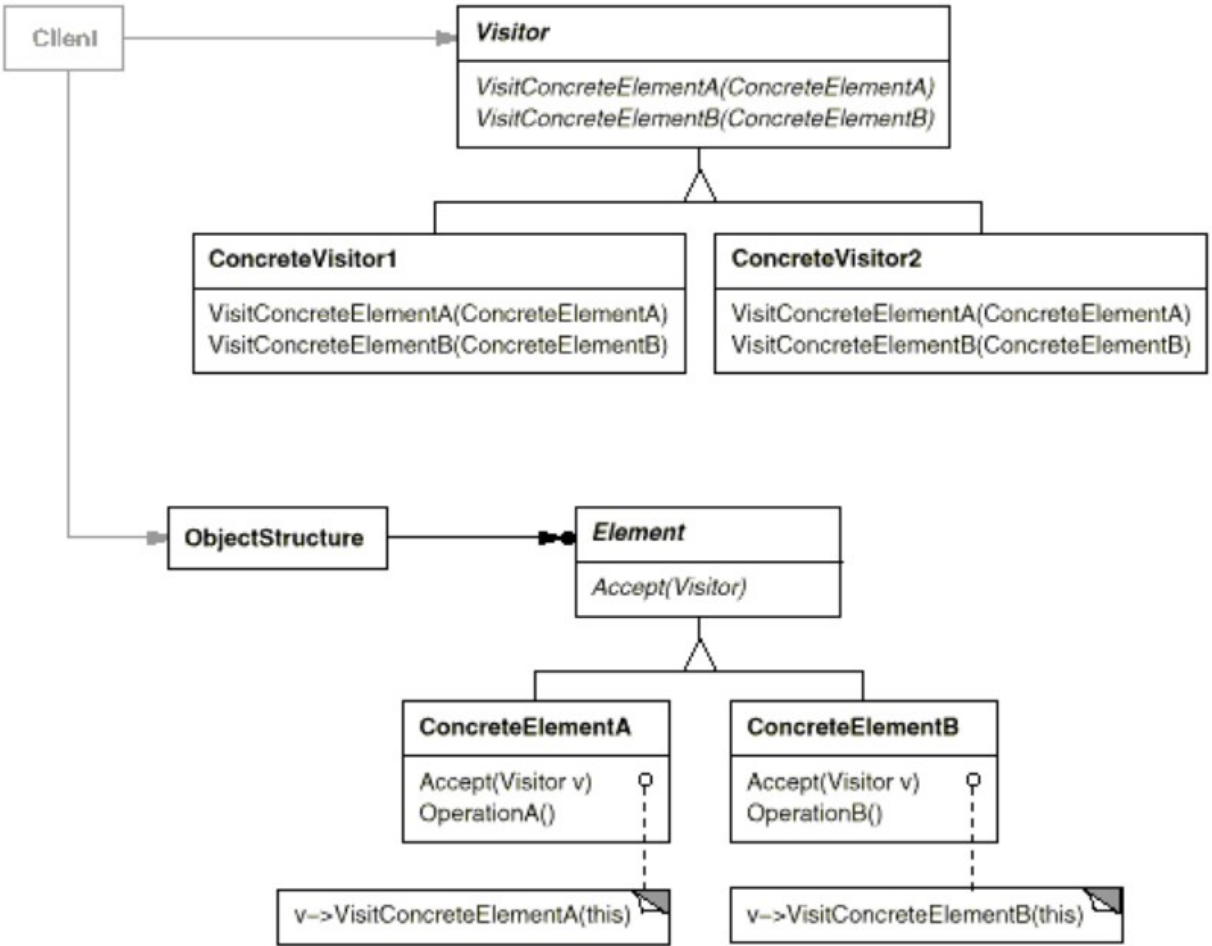
\includegraphics[width=8cm]{../../immagini/visitor/struttura_visitor}
\end{figure}

Un client crea un ConcreteVisitor e visita la struttura a oggetti.

Quando un elemento viene visitato chiama il metodo del visitor che corrisponde alla sua classe, passando se stesso come argomento, in questo modo il visitor può 
accedere allo stato dell’oggetto, se necessario.
\smallskip

Aggiungere una nuova classe alla gerarchia, come Multipliction, comporterà aggiungere un nuovo metodo visitXXX, in ExpressionVisitor, che prenderà in input 
Multipliction ed implentare accept(...) in Multipliction e l'aggiunta di questo metodo comporterà errori di compilazione nei visitor concreti, quindi occorrerà 
implementarlo.

\section{Varianti Visitor}

Supponiamo di voler rimuovere il metodo eval() da Expression e di implementare la valutazione di un espressione tramite il EvalVisitor, tale che 
EvalVisitor$<:$ExpressionVisitor.

\subsection{Visitor generico}

Dall'esempio precendete, noi sappiamo che in ExpressionVisitor i metodi visitXXX ritornano una stringa, ma a noi servirebbe che i metodi visitXXX di EvalVisitor 
ritornino un integer, quindi rendiamo ExpressionVisitor generico e, a sua volta, i metodi visitXXX e accept diventeranno generici.

Andremo a specificare l'argomento di tipo solamente quando andremo ad implementare Expression, con ParenthesisRepresentationVisitor o EvalVisitor, e nei test, in quanto
non possiamo instanziare in tipo generico, instanziamo direttamente il visitor concreto.

\subsection{Visitor void}

I metodi visitXXX e accept sono void e per questo motivo ogni visitor concreto si deve mantere uno stato, che viene usato per accumulare i risultati durante la visita, 
ed infine fornire un metodo per ottenere il risultato finale di tutta la vista.

\section{Coseguenze}

Affinchè i visitor possano agire sugli elementi, l'interfaccia degli elementi deve fornire operazioni pubbliche di accesso e questo compromette l'incapsulamento.

E' facile aggiungere nuove operazioni, basta aggiungere un visitor concreto.

E' difficile aggiungere un nuovo elemento da visitare, bisogna definire un nuovo metodo in visitor che poi dovrà essere implementato dalle classi concrete e il nuovo 
elemento da visitare deve implementare accept.

Per questo motivo, il visitor andrebbe usato quando la gerarchia degli oggetti è \underline{stabile}.

Una soluzione a questo, potrebbe essere quella di fornire un'implementazione dei metodi visitXXX in una classe astratta che implementa Visitor, cosicchè i client che 
implementeranno Visitor, estenderanno la classe astratta e ridefiniranno i metodi di loro interesse (questo però è un altro pattern).

Simulando il binding dinamico, facciamo a meno di instanceof e downcast.

Inoltre, se il linguaggio permettesse l'overloading dinamico, allora non ci sarebbe bisogno del metodo accept nelle classi da visitare ma comunque, quest'ultime, 
dovrebbero sempre fornire punti di accesso alla classe.

\end{document}

